\documentclass[a4paper,10pt]{report}
\usepackage[cm]{fullpage}
\usepackage[utf8]{inputenc}
\usepackage{amsmath}
\usepackage{amsthm}
\usepackage{amssymb}
\usepackage{appendix}
\usepackage{booktabs}
\usepackage[table]{xcolor}
\usepackage{amssymb}
\usepackage{multirow}
\usepackage{fullpage}
\usepackage{float}
\usepackage{wrapfig}
\usepackage{subfig}
\usepackage{graphicx}
\usepackage{listings}
\usepackage{color}
\usepackage{textcomp}
\usepackage{sagetex}


\usepackage{hyperref}

\definecolor{listinggray}{gray}{0.9}
%\definecolor{lbcolor}{rgb}{0.9,0.9,0.9}

\addtolength{\voffset}{-10pt}

\hypersetup{colorlinks=false}
 
\lstset{
%	backgroundcolor=\color{lbcolor},
	tabsize=4,
%	rulecolor=,
	language=python,
        basicstyle=\scriptsize,
        upquote=true,
        aboveskip={1.5\baselineskip},
        columns=fixed,
        showstringspaces=false,
        extendedchars=true,
        breaklines=true,
        prebreak = \raisebox{0ex}[0ex][0ex]{\ensuremath{\hookleftarrow}},
%        frame=single,
        showtabs=false,
        showspaces=false,
        showstringspaces=false,
        identifierstyle=\ttfamily,
        keywordstyle=\color[rgb]{0,0,1},
        commentstyle=\color[rgb]{0.133,0.545,0.133},
        stringstyle=\color[rgb]{0.627,0.126,0.941},
} \hypersetup{colorlinks=false}

\renewcommand\chaptername{Esperimento}
 
\DeclareGraphicsExtensions{.pdf,.png,.jpg}


\author{Marco Giglio, Maria Cristina Fortuna, Riccardo Iaconelli}
% Title Page
\title{Relazioni dal Laboratorio di Fisica 2}

\begin{document}

\maketitle

\tableofcontents

%INIZIALIZZAZIONE e LIBRERIE
\begin{sagesilent}
#Importo librerie necessarie
import numpy as np
from scipy import odr
import matplotlib.pyplot as plt
import matplotlib.mlab as ml
from scipy.special import chdtrc
import numpy.lib.recfunctions as rf

#classica funzione chiquadrato, non cancellare
def chiquad(xdata, ydata, yfunc, ysigma = (), param=()):
    yteo = yfunc(xdata, *param)
    ddof = len(xdata) - 1 - len(param)
    if (np.isscalar(ysigma)):
        ys = np.ones_like(xdata)*ysigma
    else:
        ys = ysigma
 
    if (len(ys)):
        return sum(((ydata-yteo)/ys)**2)
    else:
        return sum((ydata-yteo)**2/yteo)

def fit_chiquad(xdata, ydata, yfunc, init_guess, ysigma = ()):
    # Fit!
    mymodel = odr.Model(yfunc)
    mydata = odr.RealData(xdata, ydata)
    myodr = odr.ODR(mydata, mymodel, beta0=init_guess, maxit=5000)
    myout = myodr.run()
    
    # Chi^2
    yteo = yfunc(myout.beta, xdata)
    ddof = len(xdata) - 1 - len(myout.beta)

    if (np.isscalar(ysigma)):
        ys = np.ones_like(xdata)*ysigma
    else:
        ys = ysigma
 
    if (len(ys)):
        chiquad = sum(((ydata-yteo)/ys)**2)
    else:
        chiquad = sum((ydata-yteo)**2/yteo)

    prob = chdtrc(ddof,float(chiquad))
    
    return (myout, chiquad, prob)
        
#Funzione stampadati
def stampa_dati(datiarr, header):
  s = r"\begin{tabular}{c*{" + "%d" % (len(datiarr.dtype)-1)
  s += r"}{|c}}"
  s += "%s \\\\" % (header)
  s += r"\midrule"
  for i in range(0, len(datiarr)):
    a = ["%.5G" %x for x in datiarr[i]]
    s += "%s \\\\" % join(a, "&")
  s += r"\end{tabular}"
  return s
        
\end{sagesilent}



%\chapter{Misura di resistenze}

L'obiettivo del nostro esperimento è misurare la validità della legge di Ohm per varie configurazioni di un circuito. 

Al fine di misurare corrente e potenziale, colleghiamo al nostro circuito due multimetri digitali. Il primo, che ha la funzione di voltmetro, lo poniamo ai capi della nostra resistenza collegato in parallelo; il secondo, in modalità amperometro, è posto in serie subito dopo la resistenza. 

Di seguito, gli strumenti con la loro precisione:
- Voltmetro (multimetro portatile), resistenza interna: 6 $M\Omega$
- Amperometro (multimetro da banco)
- Generatore da banco, resistenza interna ignota.


\section{Analisi dati}

Ricaviamo, tramite  il fit della funzione $V=R*I$" dove R è parametro da stimare, due resistenze ignote.

\subsection{Dati}

\begin{center}
\begin{tabular}{*{4}{c}}
Corrente1 & Potenziale1 & Corrente2 & Potenziale2\\
\midrule
396 & 201 & 3043 & 207\\
512 & 261 & 3667 & 250\\
706 & 360 & 4703 & 319\\
890 & 454 & 6365 & 432\\
1126 & 574 & 8984 & 609\\
1242 & 633 & 12326 & 836\\
1557 & 794 & 16898 & 1145\\
1812 & 925 & 340 & 24\\
1971 & 1005 & 725 & 50\\
2290 & 1168 & 966 & 66\\
2524 & 1286 & 1595 & 108\\
2850 & 1454 & 1822 & 124\\
3116 & 1589 & 2160 & 146\\
3407 & 1737 & 2302 & 157\\
3883 & 1980 & 2584 & 176\\
4229 & 2157 & 3100 & 211\\
4598 & 2344 & 3370 & 229\\
5072 & 2586 & 4036 & 274\\
5505 & 2807 & 4348 & 295\\
5820 & 2967 & 4596 & 312\\
6257 & 3191 & 4894 & 332\\
6738 & 3436 & 5578 & 379\\
7521 & 3835 & 6613 & 449\\
7880 & 4018 & 6963 & 473\\
8493 & 4331 & 7371 & 500\\
8852 & 4514 & 7864 & 533\\
9135 & 4658 & 8603 & 584\\
9431 & 4809 & 9066 & 615\\
9720 & 4957 & 9667 & 656\\
9972 & 5085 & 10816 & 733\\

\end{tabular}
\end{center}


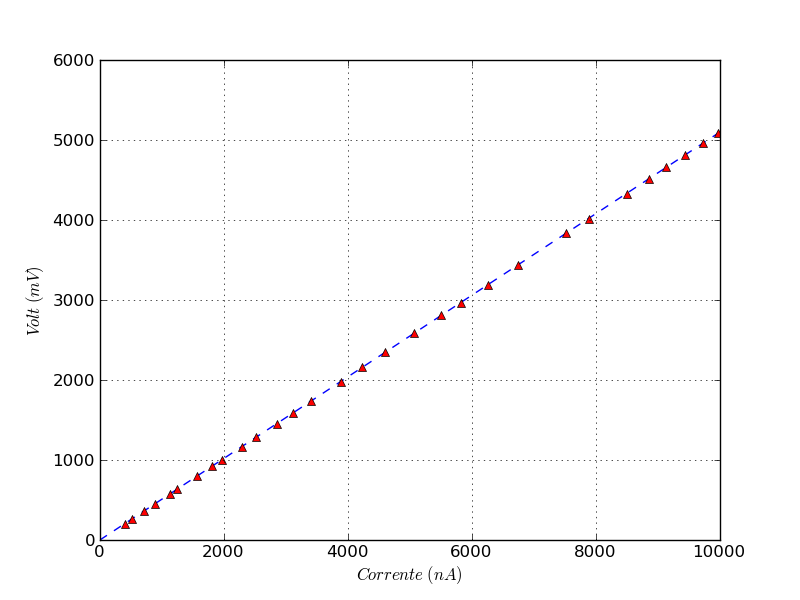
\includegraphics[scale=0.75]{grafici/C1/res1.png}
\
$\chi^2 = 5.76 $

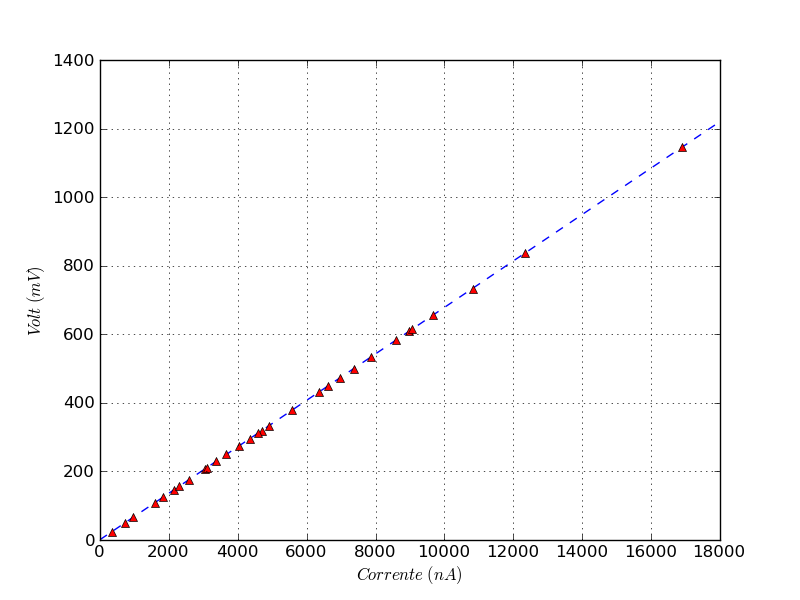
\includegraphics[scale=0.75]{grafici/C1/res2.png}

$\chi^2 = 4.88 $

Misuro la resistenza interna del voltometro, mantenendo costante la ddp a $14.5\ V$ e variando la resistenza all'interno del circuito. 
Il voltmetro è in parallelo al circuito, perciò $R_i$:

$$R_i = \frac{RV}{RI-V} $$

dove R è la resistenza variabile, I la corrente nel circuito e $V= 14.5\ V$

\begin{center}
\begin{tabular}{*{2}{c}}
Resistenza $M\Omega$ & Corrente $nA$\\
\midrule
7&      36\\
9&      32\\
10& 30\\
11&     29\\
12&     28\\
13&     27\\
14&     26\\
15&     26\\
16&     25\\
17&     24\\

\end{tabular}

La resistenza risulta $9.20 \pm 0.27 \ M \Omega$.


Misuriamo la resistenza interna dell'amperometro, che è collegato in serie al circuito. 

$$R_i = \frac{V-RI}{I}$$

In questo caso, R è fissato ($R=0.5 \Omega$) e sono V e I a variare
\begin{tabular}{*{2}{c}}
Volt $mV$ & Corrente $nA$\\
\midrule
22&      1769\\
40&      3271\\
60&      5047\\
105&     8938\\
133&     11201\\
142&     12021\\
164&     13882\\
174&     14745\\
208&     17604\\
232&     19671\\



\end{tabular}

La resistenza interna risulta $11.42 \pm 0.45 \Omega$


\end{center}


Colleghiamo una piccola lampada a filamento al circuito, e verifichiamo che il suo comportamento resistivo non segue la legge di Ohm. 

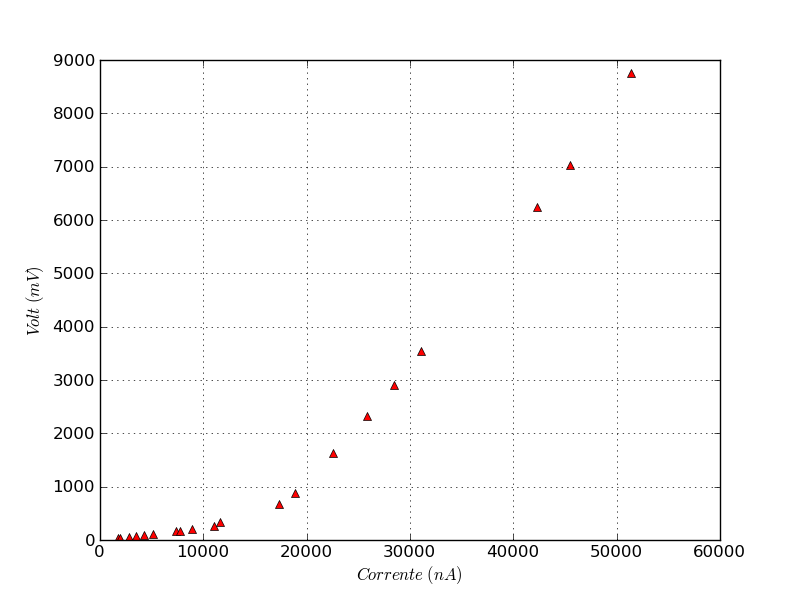
\includegraphics[scale=0.75]{grafici/C1/lampa.png}

La lampadina ha un comportamento non-ohmico nel momento in cui il filamento si scalda sufficientemente e inizia ad emettere luce ($500mV$).


\section{Partitore resistivo}

\subsection{Situazione senza carico}
\begin{center}
\begin{tabular}{*{2}{c}}
$V_{in}$ & $\frac{V_{in}}{V_{out}}$\\
\midrule
329.0 & 0.5015 \\
493.0 & 0.501 \\
544.0 & 0.5018 \\
618.0 & 0.5016 \\
667.0 & 0.5007 \\
776.0 & 0.5 \\
803.0 & 0.5006 \\
927.0 & 0.5005 \\
1078.0 & 0.5 \\
1285.0 & 0.4996 \\
\end{tabular}

\end{center}

$\chi^2=0.0169147373983$


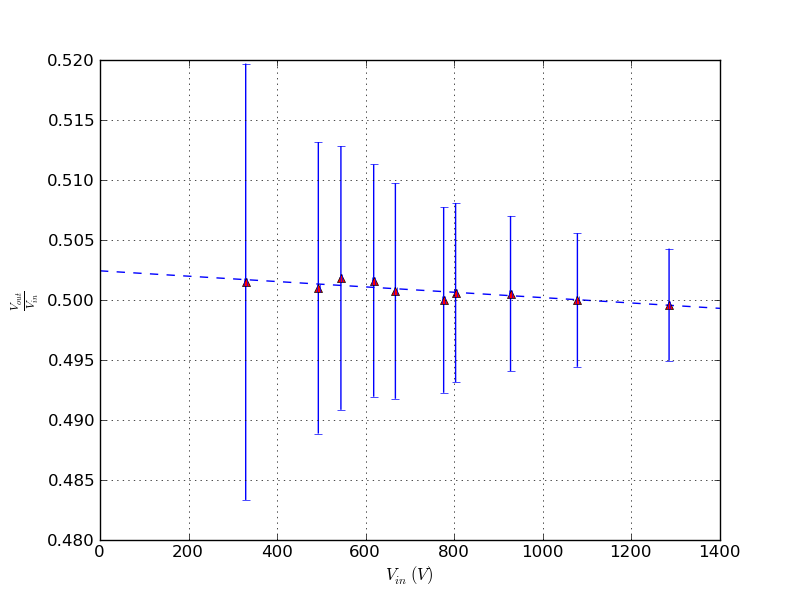
\includegraphics[scale=0.75]{grafici/C1/part1.png}

\subsection{Situazione con carico}
\begin{center}

\begin{tabular}{*{2}{c}}
$V_{in}$ & $\frac{V_{in}}{V_{out}}$\\
\midrule
220.0 & 3.1 \\
276.0 & 3.1051 \\
302.0 & 3.1126 \\
410.0 & 3.1073 \\
511.0 & 3.1115 \\
559.0 & 3.1055 \\
624.0 & 3.109 \\
752.0 & 3.109 \\
906.0 & 3.1093 \\
1036.0 & 3.111 \\
\end{tabular}

\end{center}
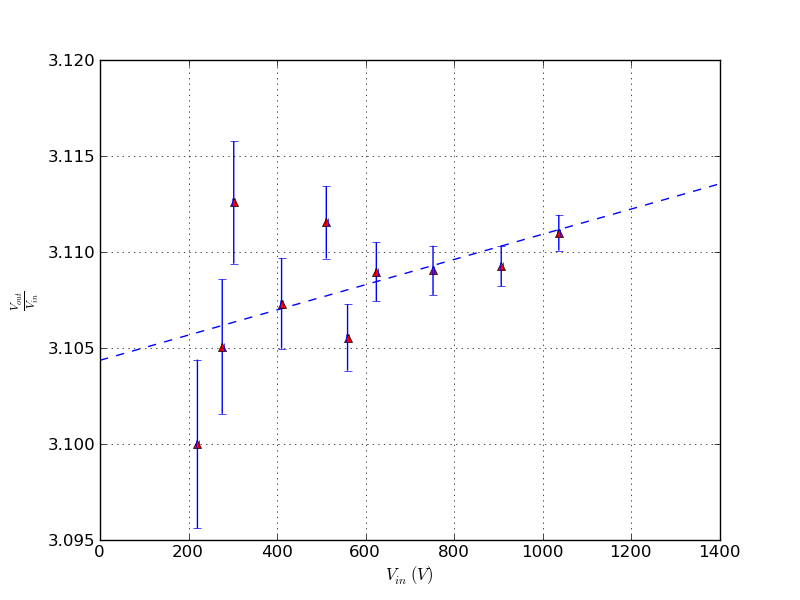
\includegraphics[scale=0.75]{grafici/C1/part2.png}

$\chi^2 = 12.9963702671$

%\begin{sagesilent}
import numpy as np

rc = np.recfromcsv("dati/C2-RC.csv")
rl = np.recfromcsv("dati/C2-RL.csv")


def stampa_dati(wa, header):
  s = r"\begin{tabular}{c*{" + "%d" % (len(wa.dtype)-1)
  s += r"}{|c}}"
  s += "%s \\\\" % (header)
  s += r"\midrule"
  for i in range(0, len(wa)):
    a = ["%s" %x for x in wa[i]]
    s += "%s \\\\" % join(a, "&")
  s += r"\end{tabular}"
  return s
\end{sagesilent}



\chapter{C2}

\section{Risposta in frequenza del multimetro}



\begin{center}
\includegraphics[scale=0.75]{grafici/C2/cv.png} 
\end{center}

Per il grafico in alto,che mostra la lettura dell'intensità di corrente in funzione della frequenza, l'errore è dato dalla sensibilità dello strumento: $\sigma_i = 0.1\ mA$.
\

Il secondo grafico, che mostra i limiti operativi del multimetro rispetto la frequenza, L'errore sulla lettura dal multimetro è la sensibilità dello strumento: $\sigma_{mu} = 0.005\ V$. Per stimare l'errore su $V_{RM}$ abbiamo usato la deviazione standard, assumendo quindi che $V_{RMS}$ dovrebbe rimanere costante. 
Indi per cui, la propagazione degli errori risulta:
$$\sigma_r = \sqrt{\frac{\sigma_{mu}^2}{V_{RMS}^2} + \frac{\sigma_{rms}^2}{V_{RMS}^4}}$$

%E' giusto pensare che rimanga costante?f'

\section{Misura di impedenze ignote}

Scopo di questa seconda parte è misurare l'impedenza di un circuito RC e RL in frequenza alternata. Mostreremo la dipendenza di Z dalla frequenza.


\begin{center}

%\sagestr{stampa_dati(rc, r"Frequenza (Hz) & I (mA) & Valore mu & $V_{rms}$ (V)")}
\end{center}


\begin{center}
\includegraphics[scale=0.75]{grafici/C2/rc.png} 
\end{center}

Dal fit ricavo: $C = 374.53\pm8.44 nF$, che rientra nei valori aspettabili, dato che il valore teorico è $367 nF$. 
Il $chi^{\tilde}^2= 1.4461 $ 

%chi quadro rotto da sistemare.

\begin{center}

%\sagestr{stampa_dati(rl, r"Frequenza (Hz) & I (mA) & Valore mu & $V_{rms}$ (V)")}
\end{center}



\begin{center}
\includegraphics[scale=0.75]{grafici/C2/rl.png} 
\end{center}

$L = 0.016074\pm 0.000092 H$
$\chi^{\tilde}^2 = 1.4546$





% \chapter{Circuiti RC e RL (C3)}

Oggetto di studio di questa esperienza è l'andamento della differenza di potenziale ai capi della resistenza e della capacità (o induttanza) di circuiti RC o RL in corrente impulsata e in corrente alternata.
A tal fine costruiamo un circuito con i seguenti elementi:

\begin{center}
 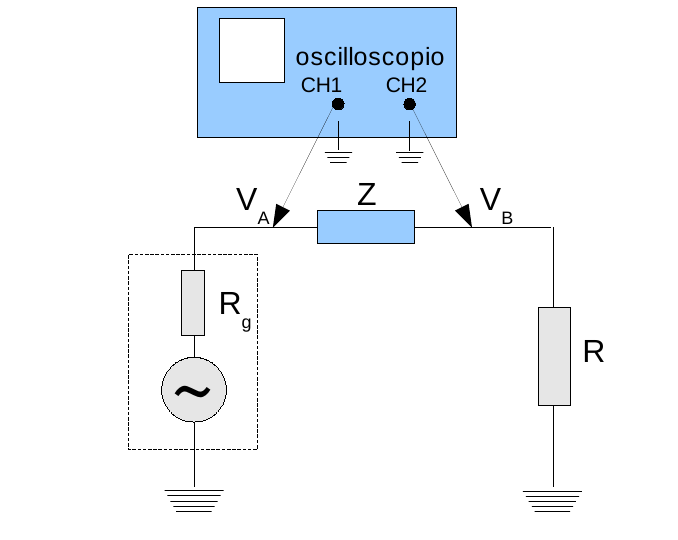
\includegraphics[scale=0.70]{grafici/C3/schema.png}
\end{center}

\begin{itemize}
  \item Generatore di onde di R= 50 $\Omega$
  \item Un condensatore di capacità 367 $nF$, misurata con il multimetro
  \item Un'induttore di induttanza sconosciuta, e resistenza 40 $\Omega$.
  \item Un oscilloscopio con due sonde
  \item Una resistenza di 677 $\Omega$ da noi misurata in C1 con un'incertezza che qui risulta trascurabile. 
\end{itemize}
La resistenza equivalente sul circuito è quindi:
\begin{itemize}
 \item Per il circuito RC: $R_{eq} = 677+50 = 727\ \Omega$.
 \item Per il circuito RL: $R_{eq} = 677+50+40 = 767\ \Omega$
\end{itemize}

\subsubsection{Nota sugli errori}
Tutte le misure di questa esperienza sono state effettuate osservando un display sul quale l'oscilloscopio rappresenta l'onda. La risoluzione (x,y) del display, dove x è l'asse temporale e y l'asse del potenziale, può essere variata a piacimento. 
Questo comporta una certa difficoltà nell'analisi degli errori. Per superarla, abbiamo notato che l'incertezza di ogni misura sulla misura stessa è un valore che rimane costante nel tempo, perchè abbiamo sempre cercato di non variare la dimensione dell'onda sullo schermo. Questo valore è tra il $4\%$ e l'$8\%$ del valore della singola misura. 


\section{Corrente impulsata: Studio del $\tau$ del circuito}

Per simulare l'apertura e la chiusura del circuito impostiamo nel generatore la modalità onda quadra. Colleghiamo la prima sonda all'ingresso del circuito, subito prima del condensatore: in tal modo l'oscilloscopio confronta il segnale in ingresso con la messa a terra, e visualizza a schermo la differenza di potenziale, restituendo sul display l'onda quadra prodotta dal generatore.  
Analogamente una seconda sonda, posta ai capi della resistenza, visualizza la forma dell'onda caratteristica della carica o della scarica del condensatore/induttore. \\
Raccogliamo i dati campionando dei punti dall'onda visualizzata sul display dell'oscilloscopio, usando i cursori per ottenere la ddp corrispondete all'istante di tempo considerato (si fissa il primo cursore sullo zero e il secondo sul punto dell'onda di cui si vuole conoscere il potenziale: l'oscilloscopio visualizza la differenza tra il potenziale dei due cursori, e dunque la ddp desiderata).
Infine interpoliamo i dati raccolti con le curve caratteristiche della carica per i due differenti circuiti, ricavando il parametro $\tau$ (tempo caratteristico dei circuiti).

\subsubsection{Circuito RC}
Con un'onda quadra a 50 Hz, abbiamo raccolto i seguenti dati:

\begin{center}
\begin{tabular}{*{2}{c}}
Tempo ($\mu s$) & Ddp ($V$) \\
\midrule
0 & 18.20 \\
100 & 12.80 \\
200 & 9.00 \\
300 & 5.80 \\
400 & 4.40 \\
500 & 3.20 \\
600 & 2.20 \\
700 & 1.80 \\
800 & 1.20 \\
900 & 1.00 \\
\end{tabular}
\end{center}

Interpoliamo i dati raccolti con la curva della carica di un condensatore: 
$$V_R = \varepsilon e^{-t/\tau}$$


%Tau per RC
\begin{sagesilent}

rct = np.recfromcsv('dati/C3/RCtau.csv')
tempo = rct['t']
volt = rct['v']
yerr = volt*0.08

def fu(P,x):
    return P[0]*exp((-1./P[1])*x)
    
def fu1(x,v,t):
    return v*exp(-x/t)
    
mymod = odr.Model(fu)
mydata = odr.RealData(tempo,volt)

myodr = odr.ODR(mydata, mymod, beta0=[20.,200.], maxit=5000)
out = myodr.run()

chi = chiquad(tempo,volt,fu1,ysigma=yerr,param=[out.beta[0],out.beta[1]])

chir = chi/(len(tempo)-2)
plt.clf()
plt.errorbar(tempo,volt,yerr,np.zeros_like(yerr),'ro')
xin = np.arange(0,1000,10)
yin = fu1(xin,out.beta[0],out.beta[1])
plt.plot(xin,yin,'--')
plt.ylabel(r"$D.d.p$ $(V)$ ")
plt.xlabel(r"$Tempo$ $(\mu s)$")
plt.grid(True)
plt.savefig("grafici/C3/RCtau.png",dpi=300)

\end{sagesilent}


\begin{center}
 \includegraphics[scale=0.70]{grafici/C3/RCtau.png}
\end{center}

Il valore stimato dall'interpolazione è $\tau=\sage{round(out.beta[1],2)}\pm \sage{round(out.sd_beta[1],2)}\ \mu s$.
Valore atteso: $\tau=RC=266.8\ \mu s$, con R=$727\ \Omega$.
L'errore è l'incertezza della misura del tempo e del potenziale, letti sul display dell'oscilloscopio. Per quanto riguarda il tempo, l'errore è stata assunto trascurabile poichè abbiamo campionato usando la griglia dell'oscilloscopio; per quanto riguarda il potenziale, abbiamo stimato un'errore percentuale del 8\%, che è circa il rapporto tra l'incertezza dello strumento e il valore della misura. 
\\
Per verificare l'accordo tra la legge e la distribuzione dei valori osservati operiamo il test del $\chi^2$:

Otteniamo $\chi^2 = \sage{round(chi,3)}$ con d.o.f = $\sage{len(tempo)-1}$\\
Il p-value associato è $0.066$, maggiore della soglia di accettabilità di $0.05$.

\subsubsection{Circuito RL}
Con un'onda quadra a 250 Hz, abbiamo raccolto i seguenti dati:

\begin{center}
\begin{tabular}{*{2}{c}}
Tempo ($\mu s$) & Ddp ($V$) \\
\midrule
5 & 5.00 \\
10 & 8.00 \\
15 & 10.60 \\
20 & 12.40 \\
25 & 13.60 \\
30 & 14.60 \\
35 & 15.40 \\
40 & 16.20 \\
45 & 16.40 \\
\end{tabular}
\end{center}
Interpoliamo i dati raccolti con la curva caratteristica della carica del circuito:

$$V_R = \varepsilon \left( 1-e^{-t/\tau} \right)$$

%Tau per RL
\begin{sagesilent}
 
rlt = np.recfromcsv('dati/C3/RLtau.csv')
tempo = rlt['t']
volt = rlt['v']
yerr = volt*0.04

def fu(P,x):
    return P[0]*(1-exp((-1./P[1])*x))
    
def fu1(x,v,t):
    return v*(1-exp(-x/t))
    
mymod = odr.Model(fu)
mydata = odr.RealData(tempo,volt)

myodr = odr.ODR(mydata, mymod, beta0=[20.,16.], maxit=5000)
out = myodr.run()

chi = chiquad(tempo,volt,fu1,ysigma=yerr,param=[out.beta[0],out.beta[1]])
dof = len(tempo)-2
chir = chi/dof

plt.clf()
plt.errorbar(tempo,volt,yerr,np.zeros_like(yerr),fmt=None)
plt.plot(tempo,volt,'ro')
xin = np.arange(min(tempo),1.5*max(tempo),1)
yin = fu1(xin,out.beta[0],out.beta[1])
plt.plot(xin,yin,'b--')
plt.ylabel(r"$D.d.p$ $(V)$ ")
plt.xlabel(r"$Tempo$ $(\mu s)$")
plt.grid(True)
plt.savefig("grafici/C3/RLtau.png",dpi=300)

\end{sagesilent}




\begin{center}
 \includegraphics[scale=0.70]{grafici/C3/RLtau.png}
\end{center}

Il valore stimato dall'interpolazione è $\tau=\sage{round(out.beta[1],2)} \pm \sage{round(out.sd_beta[1],2)}\ \mu s$. Il fit ha un $\chi^2 = \sage{round(chi,2)} $ con $d.o.f= \sage{dof}$. Il p-value associato è $0.83$.
\\

Valgono le considerazioni precedenti per quanto riguarda le incertezze. 

\section{Corrente alternata: studio frequenza di taglio}

Nella seconda parte dell'esperienza intendiamo misurare la risposta in frequenza (o funzione di trasferimento).

Pertanto misuriamo la ddp ai capi di $R$ e $C$ o $L$ in modo analogo alle prima parte dell'esperienza, e la distanza tra due picchi delle onde visualizzate a schermo per determinare l'angolo $\phi$ di sfasamento ($\delta \phi = 2 \pi \Delta t$).

Per ricavare il rapporto $\frac{V_{R}}{V_{o}}$, dobbiamo ricavare $V_R$. Trovandoci in regime di corrente alternata, la leggge di Ohm è nella forma: $ V_o = Zi_o$ con $Z = R + jX$, impedenza del circuito.
Trattandosi di circuiti RC e RL in cui le impedenze sono collegate in serie, si ha $Z_{tot} = \sum Z_i$

\begin{itemize}
\item circuito RC: $Z=R-\frac{j}{\omega C}$
\item circuito RL: $Z=R+j\omega L$
\end{itemize}  

Allora otteniamo la coppia di equazioni 

$$V_{Ro} = Ri_o = \frac{V_o}{Z} = \frac{RV_o}{\sqrt{R^2+X^2}} $$ 

$$\phi = \arctan \frac{X}{R} $$


Dove ad $X$ sostituiamo:
\begin{itemize}
\item Per il circuito RC: $X=\frac{1}{\omega C}$
\item Per il circuito RL: $X=\omega L$
\end{itemize}

Per ricavare l'opportuna funzione di trasferimento.

\subsection*{Circuito RC}


\begin{center}

\begin{tabular}{*{4}{c}}
Frequenza ($Hz$) & $V_{out}/V_{in}$ & $\phi\ (rad))$ & Delta ($\mu s$)\\
\midrule
50 & 0.08 & 1.54 & 4900\\
100 & 0.15 & 1.41 & 2240\\
200 & 0.30 & 1.41 & 1120\\
300 & 0.42 & 1.24 & 660\\
400 & 0.52 & 1.08 & 430\\
1000 & 0.83 & 0.70 & 112\\
1500 & 0.90 & 0.49 & 52\\
2000 & 0.93 & 0.38 & 30\\
4000 & 0.97 & 0.20 & 8\\

\end{tabular}
\end{center}

Lasciamo C come parametro da stimare, e interpoliamo i valori raccolti di $V_{out}$ e $V_{in}$ in funzione della frequenza, usando l'equazione:

$$\frac{V_{Ro}}{V_o} = \frac{R}{\sqrt{R^2+(\omega C)^{-2}}}$$

dove $V_{Ro} = V_{out}$ (tensione ai capi della resistenza) e $V_o = V_{in}$.

%Fit DDP per RC
\begin{sagesilent}

rcf = np.recfromcsv('dati/C3/RCfun.csv')
freq = rcf['frequenza']
freq = freq.astype(float)
vin= rcf['v_in']
volt = rcf['v_out']/rcf['v_in']
yerr = 0.01
xerr = 0

var('x,C')
def funz(x, C):
    return 727/sqrt(727^2+(x*2*n(pi)*C)^(-2))
    
def func(P,x):
    return 727/sqrt(727^2+(x*2*n(pi)*P[0])^(-2))
    
mymod = odr.Model(func)
mydata = odr.RealData(freq,volt)

myodr = odr.ODR(mydata, mymod, beta0=[0.0000001], maxit=5000)
out = myodr.run()

chi = chiquad(freq,volt,funz,ysigma=float(yerr),param=[out.beta[0]])

chir = chi/(len(freq)-1)

omega = 1/((727)*out.beta[0])
 
plt.clf()

xin = np.arange(min(freq),1.5*max(freq),10)
yin = funz(xin,out.beta[0])
plt.semilogx(freq,volt,'ro')
plt.errorbar(freq,volt,yerr,xerr,fmt=None)
plt.plot(xin,yin,'b--')
plt.ylabel(r"$\frac{V_{out}}{V_{in}}$ ")
plt.xlabel(r"$\nu$ Frequenza $(Hz)$")
plt.grid(True)
plt.savefig("grafici/C3/RCddp.png",dpi=300)
 
\end{sagesilent}


\begin{center}
 \includegraphics[scale=0.70]{grafici/C3/RCddp.png}
\end{center}

Dal fit otteniamo $C=365.42 \pm  6.11\ nF $, un $\chi^2 = \sage{round(chi,3)}$ con $d.o.f=\sage{len(freq)-1}$ e p-value: 0.25 

La frequenza di taglio è definita come $\omega_c = \frac{1}{RC}$ e per questo valore di C otteniamo $\omega_c = \sage{round(omega,2)}\ Hz$.

L'errore $\sigma_v$ deriva dagli errori su $V_{out}$ e $V_{in}$:

$\sigma_V = \sqrt{\frac{\sigma_{out}^2}{V_{in}^2} + \frac{\sigma_{in}^2}{V_{in}^4} }$

Per questa formula di propagazione, l'errore risulta irrilevante, e abbiamo stimato un'errore di $0.01 V$.
%Fit Phi per RC
\begin{sagesilent}

deltaphi= rcf['frequenza']*rcf['tempo']*2*n(pi)*10^(-6)
yerr = deltaphi*0.06
xerr= 0

var('x,C')
def funz(x, C):
    return arctan(1/(x*2*n(pi)*727*C))
    
def func(P,x):
    return arctan(1/(x*2*n(pi)*727*P[0]))
    
mymod = odr.Model(func)
mydata = odr.RealData(freq,deltaphi)

myodr = odr.ODR(mydata, mymod, beta0=[0.0000001], maxit=5000)
out = myodr.run()

chi = chiquad(freq,deltaphi,funz,ysigma=yerr,param=[out.beta[0]])

chir = chi/(len(freq)-1)

ddof=len(freq)-len(out.beta) 
 
plt.clf()

xin = np.arange(min(freq),1.5*max(freq),10)
yin = funz(xin,out.beta[0])
plt.semilogx(freq,deltaphi,'ro')
plt.errorbar(freq,deltaphi,yerr,xerr,fmt=None)
plt.plot(xin,yin,'b--')
plt.ylabel(r"$\phi (rad)$ ")
plt.xlabel(r"$\nu$ Frequenza $(Hz)$")
plt.grid(True)
plt.savefig("grafici/C3/RCfase.png",dpi=300)

omega = 1/(727*out.beta[0])
out.pprint()

\end{sagesilent}


Ora interpolo i dati della $ \phi$ utilizzando la funzione:

$$ \phi = \arctan \frac{1}{2\pi\nu C R} $$


\begin{center}
 \includegraphics[scale=0.70]{grafici/C3/RCfase.png}
\end{center}


Ricavo $C=264.90 \pm 10.1\ nF$.
Ottengo un $\chi^2 = \sage{round(chi,3)}$ con $d.o.f= \sage{len(deltaphi)-1}$ e p-value $=\sage{round(chdtrc(ddof,float(chi)),3)}$
L'errore su y è $\sigma_{y_i} = 2 \pi \nu_i \sigma_{t}$. Abbiamo supposto $\sigma_{t}$ proporzionale al tempo (è l'incertezza sulla lettura) e pari al $6\%$.
Per questo secondo valore di C, $\omega_c = \sage{round(omega,2)}\ Hz$. 

\subsubsection{Considerazioni teoriche}
Il comportamento del circuito varia a seconda di quanto la nostra frequenza $\omega$ si avvicina al valore della frequenza di taglio. \\
Per frequenze molto basse il carattere capacitivo dell'impedenza domina e pertanto la caduta di potenziale si trova tutta ai capi del condensatore, e la fase $\phi \simeq -\frac{\pi}{2}$. Viceversa per frequenze molto alte, domina il comportamento resistivo e lo sfasamento diviene: $ \phi \simeq 0$. \\  
Per $\omega \simeq \omega_c$, siamo nella transizione tra i due regimi e le impedenze si equivalgono. La fase diviene: $ \phi \simeq -\pi/4$.  \\

L'insieme dei fenomeni da noi osservati in questa secondo parte, ci permette di affermare che il circuito RC da noi costruito agisce come un filtro passa-basso passivo, cioè un filtro che riduce le componenti alle frequenze superiori a quella di taglio (abbattendo l'ampiezza di $V_{out}$ all'aumentare della frequenza, come si vede nel grafico). Il più semplice filtro passa-basso è, infatti, un circuito RC. 

\subsection*{Circuito RL}
\begin{center}

\begin{tabular}{*{4}{c}}
Frequenza ($Hz$) & Delta V ($V_{out}/V_{in}$) & $\phi (rad)$ & Delta ($\mu s$) \\
\midrule
1000& 0.47 & 0.19 & 30 \\
2000 & 0.62 & 0.35 & 28\\
3000 & 0.79 & 0.45 & 24\\
4000 & 1.05 & 0.58 & 23\\
6000 & 1.48 & 0.79 & 21\\
8000 & 2.01 & 1.01 & 20\\
10000 & 2.56 & 0.94 & 15\\
15000 & 3.64 & 1.13 & 12\\
20000 & 4.28 & 1.26 & 10 \\
30000 & 5.08 & 1.36 & 7.2\\
50000 & 5.89 & 1.57 & 5\\
\end{tabular}
\end{center}



Anche questa volta interpoliamo i dati raccolti con la funzione:

$$\frac{V_{Ro}}{V_o} = \frac{R}{\sqrt{R^2+(\omega L)^2}}$$


%Fit DDP per RL
\begin{sagesilent}

#Fit del ddp in funzione della frequenza per l'induttore
dati3 = np.recfromcsv('dati/C3/RLfun.csv',delimiter="\t")
dati3 = np.sort(dati3)

deltaV = dati3['v_out']/dati3['v_in']
yerr = 0.05
xerr= 0

var('x,L')

def func(x, L):
    return (767/(np.sqrt((767)^2+(x*2*n(pi)*L)^2)))

def fu(P, x):
    return func(x, P[0])
 
import scipy.odr as odr
mymodel = odr.Model(fu)
mydata = odr.RealData(dati3['frequenza'], deltaV)
myodr = odr.ODR(mydata, mymodel, beta0=[0.002],  maxit=1000)
myout = myodr.run()

chiquadrato = chiquad(np.array(dati3['frequenza']), deltaV, fu, ysigma=float(0.1), param=[myout.beta])

plt.clf()
plt.semilogx(dati3['frequenza'],deltaV , 'ro')
xsp = np.arange(0, 500000, 500)
ysp = func(xsp, myout.beta[0])
plt.plot(xsp, ysp, 'b--')
plt.errorbar(dati3['frequenza'],deltaV,yerr,xerr,fmt=None)
plt.grid(True)
plt.ylabel(r"$\frac{V_{out}}{V_{in}}$ ")
plt.xlabel(r"Frequenza $\nu$ - $(Hz)$")
plt.savefig("grafici/C3/RLddp.png", dpi=300)
omega = 767/myout.beta[0]
lstring = "%.4G" % (myout.beta[0]*1000)
lerrorstring = "%.2G" % (myout.sd_beta[0]*1000)
\end{sagesilent}

\begin{center}
 \includegraphics[scale=0.70]{grafici/C3/RLddp.png}
\end{center}



Otteniamo $L=\sage{lstring}\pm\sage{lerrorstring} \ H$.  Non ha senso calcolare il $\chi^2$, poichè la funzione di fit non è in buon accordo con i nostri dati. Sospettiamo la presenza di impedenze ignote che abbiamo trascurato.


La frequenza di taglio viene definita come $\omega_c = R/L$. Usando la L di questo fit, $\omega_c = \sage{round(omega,2)}\ Hz$. 

%Fit Phi per RL
\begin{sagesilent}

rlf = np.recfromcsv('dati/C3/RLfun.csv',delimiter="\t")
freq = rlf['frequenza']
deltaphi= rlf['frequenza']*rlf['delta']*2*n(pi)*10^(-6)
yerr = deltaphi*0.06
xerr= 0

var('x,L')
def funz(x, L):
    return arctan(x*2*n(pi)*L/767)
    
def func(P,x):
    return arctan(x*2*n(pi)*P[0]/767)
    
mymod = odr.Model(func)
mydata = odr.RealData(freq,deltaphi)

myodr = odr.ODR(mydata, mymod, beta0=[0.012], maxit=1000)
out = myodr.run()

chi = chiquad(freq,deltaphi,funz,ysigma=yerr,param=[out.beta[0]])

chir = chi/(len(freq)-1)
 
plt.clf()

xin = np.arange(0.5*min(freq),1.5*max(freq),10)
yin = funz(xin,out.beta[0])
plt.semilogx(freq,deltaphi,'ro')
plt.errorbar(freq,deltaphi,yerr,xerr,fmt=None)
plt.plot(xin,yin,'b--')
plt.ylabel(r"$\phi (rad)$ ")
plt.xlabel(r"$\nu$ Frequenza $(Hz)$")
plt.grid(True)
plt.savefig("grafici/C3/RLfase.png",dpi=300)
out.pprint()
omega = 767/(out.beta[0])

\end{sagesilent}


Interpolo i dati della $\phi$, utilizzando la funzione:

$$ \phi = \arctan \frac{2\pi\nu L}{R} $$

dove L è il parametro libero da stimare.

\begin{center}
 \includegraphics[scale=0.70]{grafici/C3/RLfase.png}
\end{center}


$L=20.2\pm0.01\ mH$. Il fit ha un $\chi^2 = \sage{round(chi,2)}$ con $d.o.f= \sage{len(freq)-1}$ e p-value:0.18. Per l'analisi degli errori, valgono le considerazioni fatte in precedenza per il circuito RC.\\

La frequenza di taglio viene definita come $\omega_c = R/L$. Usando la L di questo fit, $\omega_c = \sage{round(omega,2)}\ Hz$. 
\\
\subsubsection{Considerazioni teoriche}
Il comportamento del nostro circuito varia a seconda di quanto la nostra frequenza $\omega$ si avvicina al valore della frequenza di taglio. \\
Per frequenze molto basse il carattere resistivo dell'impedenza domina e pertanto la caduta di potenziale si trova solo ai capi della resistenza; per cui $ \phi \simeq 0$. Viceversa per frequenze molto alte, domina il comportamento induttivo, e lo sfasamento prodotto è simile a quello che introdurrebbe nel circuito un componente puramente induttivo ($\phi \simeq \frac{\pi}{2}$).  \\
Per $\omega = \omega_c$, essendo in transizione tra i due regime, si ha un comportamento intermedio e la fase diviene: $ \phi = \pi/4$. \\

L'insieme dei fenomeni da noi osservati in questa secondo parte, ci permette di affermare che il circuito RL da noi costruito agisce come un filtro passa-alto passivo, cioè un filtro che riduce le componenti alle frequenze inferiori a quella di taglio (abbattendo l'ampiezza di $V_{out}$ al diminuire della frequenza , come si vede nel grafico). Il più semplice filtro passa-alto è, infatti, un circuito RL. 

% \chapter{C4}

\begin{sagesilent}

import numpy as np
from scipy import odr
import matplotlib.pyplot as plt

trasfm = np.recfromcsv("dati/C4-tensione-fase.csv")

#Sottosmorzamento tempo-volt
#Smorzamento critico tempo-volt
#Sovrasmorzamento tempo-volt
\end{sagesilent}


\begin{sagesilent}

#Funzione di trasferimento del modulo: freq-volt
#RLC in corrente alternata
dati = np.recfromcsv("dati/C4-tensione-fase.csv")
var('x,l,c,v,w')
r = 300
def f(x, l, w, v):
    return (v*2*3.14*x*w)/( sqrt( (2*3.14*x*w)^2+(w*l/r)^2*((2*3.14*x)^2-w^2)^2 ) )
    
puls = dati['frequenza_hz'] #*2*3.14
ennupla = list(((puls[i]), dati['v_out__v_in'][i]) for i in range(0,len(dati['frequenza_hz'])))


fit = find_fit(ennupla, f, parameters=[l,w,v], variables=[x], solution_dict=True)

print fit

plt.clf()
xin = np.arange(100, 100000, 10)
yin = f(xin, fit[l], fit[w], fit[v])
plt.semilogx(xin,yin, 'g--')
plt.semilogx(dati['frequenza_hz'], dati['v_out__v_in'], 'ok')

plt.xlabel(r"$\omega$ [$rad/s$]")
plt.ylabel(r"$V(\omega)$ [$rad$]")
plt.grid(True)

plt.savefig("grafici/C4-ris.png", dpi=300)

#Funzione di trasferimento fase:freq-rad
  
\end{sagesilent}

\includegraphics[scale=0.75]{grafici/C4-ris.png}



%Sottosmorzamento
\begin{sagesilent}
 
om = 2*n(pi)*100
t =np.array([190,570,950,1520])
picchi=np.array([520,-148,60,-24])

def func(P,x):
    return P[0]*P[1]*P[2]*exp(-P[3]*t)*(P[3]*cos(om*x)+om*sin(100*x))

#var('x,r,c,v,g')
#def f(x,r,c, v, g):
#    return r*c*v*exp(-g*t)*(g*cos(om*x)+om*sin(100*x))
    
plt.clf()
plt.plot(t,picchi,'bo')

mod = odr.Model(func)
data = odr.RealData(t,picchi)
done = odr.ODR(data, mod, beta0=[1.,1.,1.,1.],maxit=1000)
sotto = done.run()

#xin = np.arange(min(t),max(t),1)
#yin = func(sotto.beta, xin)

#plt.plot(xin,yin,'g--')
plt.xlabel(r"$\omega$ [$rad/s$]")
plt.ylabel(r"$V(\omega)$ [$rad$]")
plt.savefig("grafici/C4-om.png",dpi=300)
 
\end{sagesilent}

\begin{center}
 \includegraphics[scale=0.75]{grafici/C4-om.png}
\end{center}

%Funzione di trasferimento del modulo
% \begin{sagesilent}
% 
% freq = trasfm['frequenza_hz']
% v = trasfm['v_out_v_in']
% 
% #Funzione di trasferimento del modulo
% 
% def fu(P,x):
%     return (P[0]*2*3.14*x*P[1])/( sqrt( (2*3.14*x*P[1])^2+(w*P[2]/R)^2*((2*3.14*x)^2-[1]^2)^2 ) )
% 
%   
% myodr, chi = fit_chiquad(freq, v, fu, ysigma=yerr, param=[mytransm.beta])
% print "Chi quadro %.4f" % chi
%   
% \end{sagesilent}


 %\chapter{Misura di resistenze}

L'obiettivo del nostro esperimento è misurare la validità della legge di Ohm per varie configurazioni di un circuito. 

Al fine di misurare corrente e potenziale, colleghiamo al nostro circuito due multimetri digitali. Il primo, che ha la funzione di voltmetro, lo poniamo ai capi della nostra resistenza collegato in parallelo; il secondo, in modalità amperometro, è posto in serie subito dopo la resistenza. 

Di seguito, gli strumenti con la loro precisione:
- Voltmetro (multimetro portatile), resistenza interna: 6 $M\Omega$
- Amperometro (multimetro da banco)
- Generatore da banco, resistenza interna ignota.


\section{Analisi dati}

Ricaviamo, tramite  il fit della funzione $V=R*I$" dove R è parametro da stimare, due resistenze ignote.

\subsection{Dati}

\begin{center}
\begin{tabular}{*{4}{c}}
Corrente1 & Potenziale1 & Corrente2 & Potenziale2\\
\midrule
396 & 201 & 3043 & 207\\
512 & 261 & 3667 & 250\\
706 & 360 & 4703 & 319\\
890 & 454 & 6365 & 432\\
1126 & 574 & 8984 & 609\\
1242 & 633 & 12326 & 836\\
1557 & 794 & 16898 & 1145\\
1812 & 925 & 340 & 24\\
1971 & 1005 & 725 & 50\\
2290 & 1168 & 966 & 66\\
2524 & 1286 & 1595 & 108\\
2850 & 1454 & 1822 & 124\\
3116 & 1589 & 2160 & 146\\
3407 & 1737 & 2302 & 157\\
3883 & 1980 & 2584 & 176\\
4229 & 2157 & 3100 & 211\\
4598 & 2344 & 3370 & 229\\
5072 & 2586 & 4036 & 274\\
5505 & 2807 & 4348 & 295\\
5820 & 2967 & 4596 & 312\\
6257 & 3191 & 4894 & 332\\
6738 & 3436 & 5578 & 379\\
7521 & 3835 & 6613 & 449\\
7880 & 4018 & 6963 & 473\\
8493 & 4331 & 7371 & 500\\
8852 & 4514 & 7864 & 533\\
9135 & 4658 & 8603 & 584\\
9431 & 4809 & 9066 & 615\\
9720 & 4957 & 9667 & 656\\
9972 & 5085 & 10816 & 733\\

\end{tabular}
\end{center}


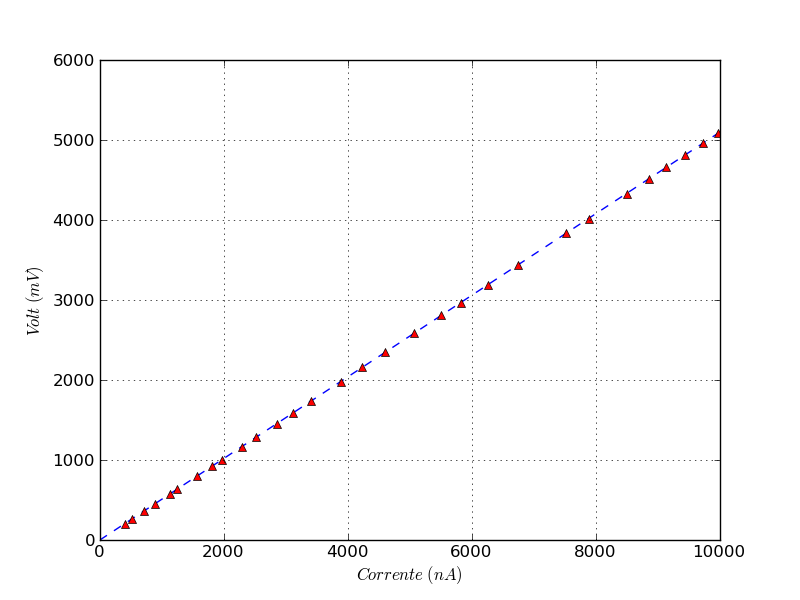
\includegraphics[scale=0.75]{grafici/C1/res1.png}
\
$\chi^2 = 5.76 $

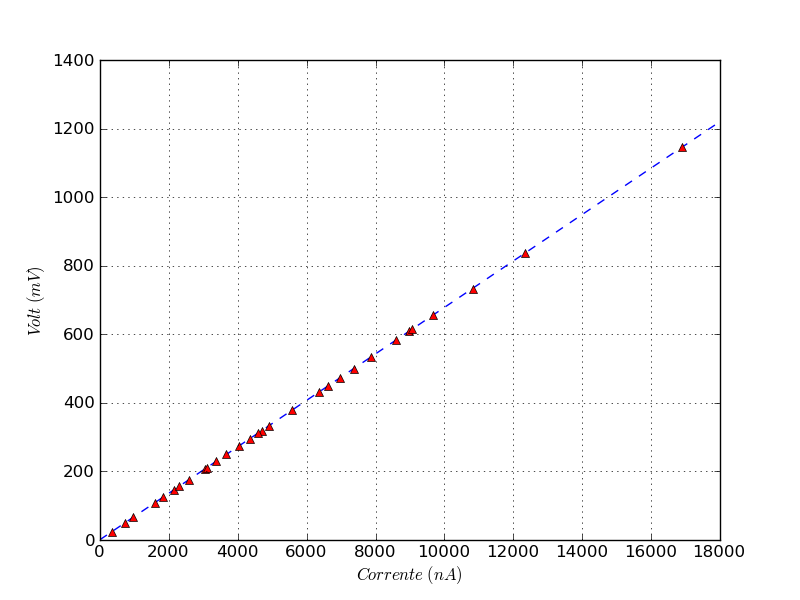
\includegraphics[scale=0.75]{grafici/C1/res2.png}

$\chi^2 = 4.88 $

Misuro la resistenza interna del voltometro, mantenendo costante la ddp a $14.5\ V$ e variando la resistenza all'interno del circuito. 
Il voltmetro è in parallelo al circuito, perciò $R_i$:

$$R_i = \frac{RV}{RI-V} $$

dove R è la resistenza variabile, I la corrente nel circuito e $V= 14.5\ V$

\begin{center}
\begin{tabular}{*{2}{c}}
Resistenza $M\Omega$ & Corrente $nA$\\
\midrule
7&      36\\
9&      32\\
10& 30\\
11&     29\\
12&     28\\
13&     27\\
14&     26\\
15&     26\\
16&     25\\
17&     24\\

\end{tabular}

La resistenza risulta $9.20 \pm 0.27 \ M \Omega$.


Misuriamo la resistenza interna dell'amperometro, che è collegato in serie al circuito. 

$$R_i = \frac{V-RI}{I}$$

In questo caso, R è fissato ($R=0.5 \Omega$) e sono V e I a variare
\begin{tabular}{*{2}{c}}
Volt $mV$ & Corrente $nA$\\
\midrule
22&      1769\\
40&      3271\\
60&      5047\\
105&     8938\\
133&     11201\\
142&     12021\\
164&     13882\\
174&     14745\\
208&     17604\\
232&     19671\\



\end{tabular}

La resistenza interna risulta $11.42 \pm 0.45 \Omega$


\end{center}


Colleghiamo una piccola lampada a filamento al circuito, e verifichiamo che il suo comportamento resistivo non segue la legge di Ohm. 

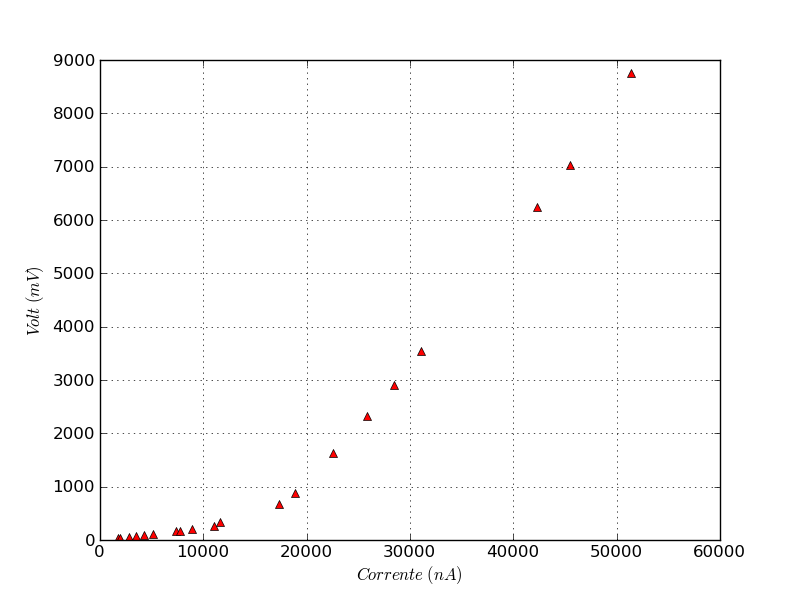
\includegraphics[scale=0.75]{grafici/C1/lampa.png}

La lampadina ha un comportamento non-ohmico nel momento in cui il filamento si scalda sufficientemente e inizia ad emettere luce ($500mV$).


\section{Partitore resistivo}

\subsection{Situazione senza carico}
\begin{center}
\begin{tabular}{*{2}{c}}
$V_{in}$ & $\frac{V_{in}}{V_{out}}$\\
\midrule
329.0 & 0.5015 \\
493.0 & 0.501 \\
544.0 & 0.5018 \\
618.0 & 0.5016 \\
667.0 & 0.5007 \\
776.0 & 0.5 \\
803.0 & 0.5006 \\
927.0 & 0.5005 \\
1078.0 & 0.5 \\
1285.0 & 0.4996 \\
\end{tabular}

\end{center}

$\chi^2=0.0169147373983$


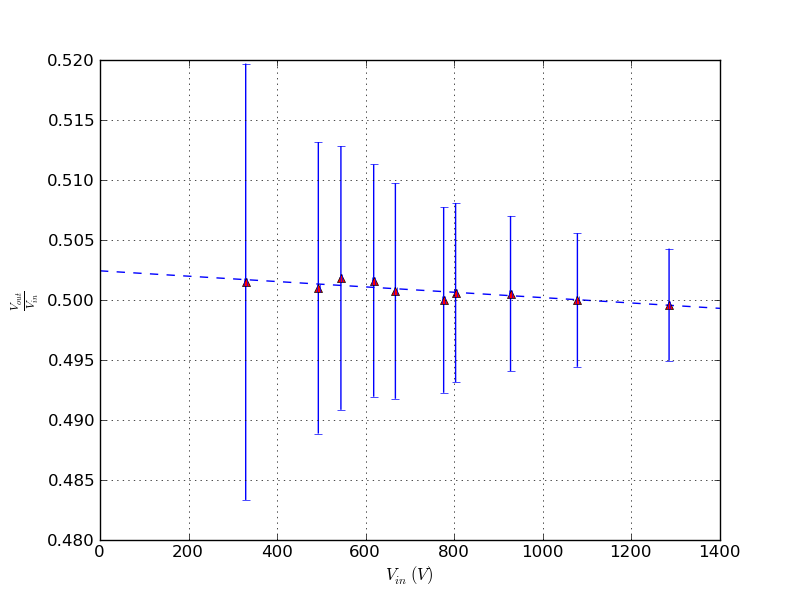
\includegraphics[scale=0.75]{grafici/C1/part1.png}

\subsection{Situazione con carico}
\begin{center}

\begin{tabular}{*{2}{c}}
$V_{in}$ & $\frac{V_{in}}{V_{out}}$\\
\midrule
220.0 & 3.1 \\
276.0 & 3.1051 \\
302.0 & 3.1126 \\
410.0 & 3.1073 \\
511.0 & 3.1115 \\
559.0 & 3.1055 \\
624.0 & 3.109 \\
752.0 & 3.109 \\
906.0 & 3.1093 \\
1036.0 & 3.111 \\
\end{tabular}

\end{center}
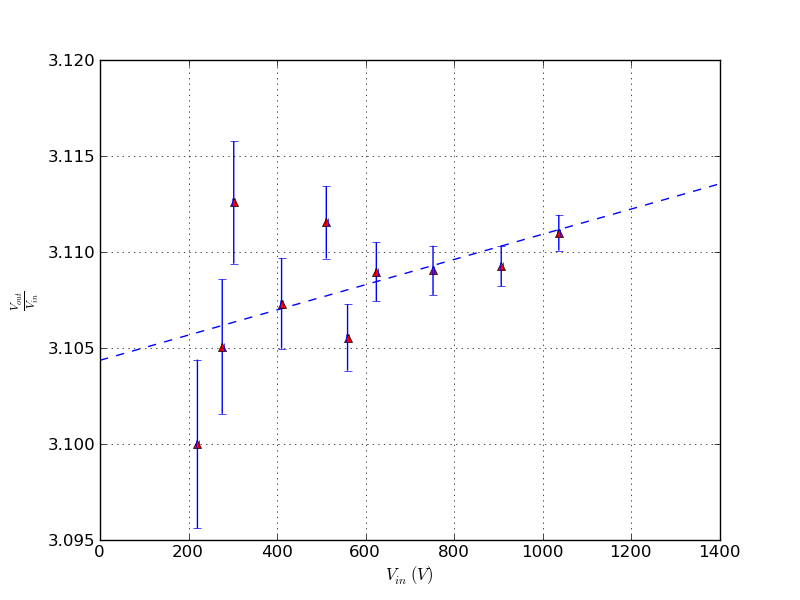
\includegraphics[scale=0.75]{grafici/C1/part2.png}

$\chi^2 = 12.9963702671$

% \begin{sagesilent}
import numpy as np

rc = np.recfromcsv("dati/C2-RC.csv")
rl = np.recfromcsv("dati/C2-RL.csv")


def stampa_dati(wa, header):
  s = r"\begin{tabular}{c*{" + "%d" % (len(wa.dtype)-1)
  s += r"}{|c}}"
  s += "%s \\\\" % (header)
  s += r"\midrule"
  for i in range(0, len(wa)):
    a = ["%s" %x for x in wa[i]]
    s += "%s \\\\" % join(a, "&")
  s += r"\end{tabular}"
  return s
\end{sagesilent}



\chapter{C2}

\section{Risposta in frequenza del multimetro}



\begin{center}
\includegraphics[scale=0.75]{grafici/C2/cv.png} 
\end{center}

Per il grafico in alto,che mostra la lettura dell'intensità di corrente in funzione della frequenza, l'errore è dato dalla sensibilità dello strumento: $\sigma_i = 0.1\ mA$.
\

Il secondo grafico, che mostra i limiti operativi del multimetro rispetto la frequenza, L'errore sulla lettura dal multimetro è la sensibilità dello strumento: $\sigma_{mu} = 0.005\ V$. Per stimare l'errore su $V_{RM}$ abbiamo usato la deviazione standard, assumendo quindi che $V_{RMS}$ dovrebbe rimanere costante. 
Indi per cui, la propagazione degli errori risulta:
$$\sigma_r = \sqrt{\frac{\sigma_{mu}^2}{V_{RMS}^2} + \frac{\sigma_{rms}^2}{V_{RMS}^4}}$$

%E' giusto pensare che rimanga costante?f'

\section{Misura di impedenze ignote}

Scopo di questa seconda parte è misurare l'impedenza di un circuito RC e RL in frequenza alternata. Mostreremo la dipendenza di Z dalla frequenza.


\begin{center}

%\sagestr{stampa_dati(rc, r"Frequenza (Hz) & I (mA) & Valore mu & $V_{rms}$ (V)")}
\end{center}


\begin{center}
\includegraphics[scale=0.75]{grafici/C2/rc.png} 
\end{center}

Dal fit ricavo: $C = 374.53\pm8.44 nF$, che rientra nei valori aspettabili, dato che il valore teorico è $367 nF$. 
Il $chi^{\tilde}^2= 1.4461 $ 

%chi quadro rotto da sistemare.

\begin{center}

%\sagestr{stampa_dati(rl, r"Frequenza (Hz) & I (mA) & Valore mu & $V_{rms}$ (V)")}
\end{center}



\begin{center}
\includegraphics[scale=0.75]{grafici/C2/rl.png} 
\end{center}

$L = 0.016074\pm 0.000092 H$
$\chi^{\tilde}^2 = 1.4546$





% \chapter{Circuiti RC e RL (C3)}

Oggetto di studio di questa esperienza è l'andamento della differenza di potenziale ai capi della resistenza e della capacità (o induttanza) di circuiti RC o RL in corrente impulsata e in corrente alternata.
A tal fine costruiamo un circuito con i seguenti elementi:

\begin{center}
 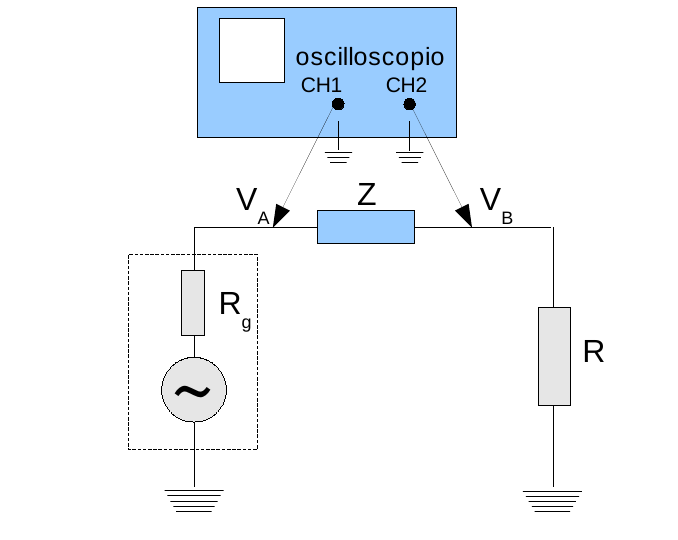
\includegraphics[scale=0.70]{grafici/C3/schema.png}
\end{center}

\begin{itemize}
  \item Generatore di onde di R= 50 $\Omega$
  \item Un condensatore di capacità 367 $nF$, misurata con il multimetro
  \item Un'induttore di induttanza sconosciuta, e resistenza 40 $\Omega$.
  \item Un oscilloscopio con due sonde
  \item Una resistenza di 677 $\Omega$ da noi misurata in C1 con un'incertezza che qui risulta trascurabile. 
\end{itemize}
La resistenza equivalente sul circuito è quindi:
\begin{itemize}
 \item Per il circuito RC: $R_{eq} = 677+50 = 727\ \Omega$.
 \item Per il circuito RL: $R_{eq} = 677+50+40 = 767\ \Omega$
\end{itemize}

\subsubsection{Nota sugli errori}
Tutte le misure di questa esperienza sono state effettuate osservando un display sul quale l'oscilloscopio rappresenta l'onda. La risoluzione (x,y) del display, dove x è l'asse temporale e y l'asse del potenziale, può essere variata a piacimento. 
Questo comporta una certa difficoltà nell'analisi degli errori. Per superarla, abbiamo notato che l'incertezza di ogni misura sulla misura stessa è un valore che rimane costante nel tempo, perchè abbiamo sempre cercato di non variare la dimensione dell'onda sullo schermo. Questo valore è tra il $4\%$ e l'$8\%$ del valore della singola misura. 


\section{Corrente impulsata: Studio del $\tau$ del circuito}

Per simulare l'apertura e la chiusura del circuito impostiamo nel generatore la modalità onda quadra. Colleghiamo la prima sonda all'ingresso del circuito, subito prima del condensatore: in tal modo l'oscilloscopio confronta il segnale in ingresso con la messa a terra, e visualizza a schermo la differenza di potenziale, restituendo sul display l'onda quadra prodotta dal generatore.  
Analogamente una seconda sonda, posta ai capi della resistenza, visualizza la forma dell'onda caratteristica della carica o della scarica del condensatore/induttore. \\
Raccogliamo i dati campionando dei punti dall'onda visualizzata sul display dell'oscilloscopio, usando i cursori per ottenere la ddp corrispondete all'istante di tempo considerato (si fissa il primo cursore sullo zero e il secondo sul punto dell'onda di cui si vuole conoscere il potenziale: l'oscilloscopio visualizza la differenza tra il potenziale dei due cursori, e dunque la ddp desiderata).
Infine interpoliamo i dati raccolti con le curve caratteristiche della carica per i due differenti circuiti, ricavando il parametro $\tau$ (tempo caratteristico dei circuiti).

\subsubsection{Circuito RC}
Con un'onda quadra a 50 Hz, abbiamo raccolto i seguenti dati:

\begin{center}
\begin{tabular}{*{2}{c}}
Tempo ($\mu s$) & Ddp ($V$) \\
\midrule
0 & 18.20 \\
100 & 12.80 \\
200 & 9.00 \\
300 & 5.80 \\
400 & 4.40 \\
500 & 3.20 \\
600 & 2.20 \\
700 & 1.80 \\
800 & 1.20 \\
900 & 1.00 \\
\end{tabular}
\end{center}

Interpoliamo i dati raccolti con la curva della carica di un condensatore: 
$$V_R = \varepsilon e^{-t/\tau}$$


%Tau per RC
\begin{sagesilent}

rct = np.recfromcsv('dati/C3/RCtau.csv')
tempo = rct['t']
volt = rct['v']
yerr = volt*0.08

def fu(P,x):
    return P[0]*exp((-1./P[1])*x)
    
def fu1(x,v,t):
    return v*exp(-x/t)
    
mymod = odr.Model(fu)
mydata = odr.RealData(tempo,volt)

myodr = odr.ODR(mydata, mymod, beta0=[20.,200.], maxit=5000)
out = myodr.run()

chi = chiquad(tempo,volt,fu1,ysigma=yerr,param=[out.beta[0],out.beta[1]])

chir = chi/(len(tempo)-2)
plt.clf()
plt.errorbar(tempo,volt,yerr,np.zeros_like(yerr),'ro')
xin = np.arange(0,1000,10)
yin = fu1(xin,out.beta[0],out.beta[1])
plt.plot(xin,yin,'--')
plt.ylabel(r"$D.d.p$ $(V)$ ")
plt.xlabel(r"$Tempo$ $(\mu s)$")
plt.grid(True)
plt.savefig("grafici/C3/RCtau.png",dpi=300)

\end{sagesilent}


\begin{center}
 \includegraphics[scale=0.70]{grafici/C3/RCtau.png}
\end{center}

Il valore stimato dall'interpolazione è $\tau=\sage{round(out.beta[1],2)}\pm \sage{round(out.sd_beta[1],2)}\ \mu s$.
Valore atteso: $\tau=RC=266.8\ \mu s$, con R=$727\ \Omega$.
L'errore è l'incertezza della misura del tempo e del potenziale, letti sul display dell'oscilloscopio. Per quanto riguarda il tempo, l'errore è stata assunto trascurabile poichè abbiamo campionato usando la griglia dell'oscilloscopio; per quanto riguarda il potenziale, abbiamo stimato un'errore percentuale del 8\%, che è circa il rapporto tra l'incertezza dello strumento e il valore della misura. 
\\
Per verificare l'accordo tra la legge e la distribuzione dei valori osservati operiamo il test del $\chi^2$:

Otteniamo $\chi^2 = \sage{round(chi,3)}$ con d.o.f = $\sage{len(tempo)-1}$\\
Il p-value associato è $0.066$, maggiore della soglia di accettabilità di $0.05$.

\subsubsection{Circuito RL}
Con un'onda quadra a 250 Hz, abbiamo raccolto i seguenti dati:

\begin{center}
\begin{tabular}{*{2}{c}}
Tempo ($\mu s$) & Ddp ($V$) \\
\midrule
5 & 5.00 \\
10 & 8.00 \\
15 & 10.60 \\
20 & 12.40 \\
25 & 13.60 \\
30 & 14.60 \\
35 & 15.40 \\
40 & 16.20 \\
45 & 16.40 \\
\end{tabular}
\end{center}
Interpoliamo i dati raccolti con la curva caratteristica della carica del circuito:

$$V_R = \varepsilon \left( 1-e^{-t/\tau} \right)$$

%Tau per RL
\begin{sagesilent}
 
rlt = np.recfromcsv('dati/C3/RLtau.csv')
tempo = rlt['t']
volt = rlt['v']
yerr = volt*0.04

def fu(P,x):
    return P[0]*(1-exp((-1./P[1])*x))
    
def fu1(x,v,t):
    return v*(1-exp(-x/t))
    
mymod = odr.Model(fu)
mydata = odr.RealData(tempo,volt)

myodr = odr.ODR(mydata, mymod, beta0=[20.,16.], maxit=5000)
out = myodr.run()

chi = chiquad(tempo,volt,fu1,ysigma=yerr,param=[out.beta[0],out.beta[1]])
dof = len(tempo)-2
chir = chi/dof

plt.clf()
plt.errorbar(tempo,volt,yerr,np.zeros_like(yerr),fmt=None)
plt.plot(tempo,volt,'ro')
xin = np.arange(min(tempo),1.5*max(tempo),1)
yin = fu1(xin,out.beta[0],out.beta[1])
plt.plot(xin,yin,'b--')
plt.ylabel(r"$D.d.p$ $(V)$ ")
plt.xlabel(r"$Tempo$ $(\mu s)$")
plt.grid(True)
plt.savefig("grafici/C3/RLtau.png",dpi=300)

\end{sagesilent}




\begin{center}
 \includegraphics[scale=0.70]{grafici/C3/RLtau.png}
\end{center}

Il valore stimato dall'interpolazione è $\tau=\sage{round(out.beta[1],2)} \pm \sage{round(out.sd_beta[1],2)}\ \mu s$. Il fit ha un $\chi^2 = \sage{round(chi,2)} $ con $d.o.f= \sage{dof}$. Il p-value associato è $0.83$.
\\

Valgono le considerazioni precedenti per quanto riguarda le incertezze. 

\section{Corrente alternata: studio frequenza di taglio}

Nella seconda parte dell'esperienza intendiamo misurare la risposta in frequenza (o funzione di trasferimento).

Pertanto misuriamo la ddp ai capi di $R$ e $C$ o $L$ in modo analogo alle prima parte dell'esperienza, e la distanza tra due picchi delle onde visualizzate a schermo per determinare l'angolo $\phi$ di sfasamento ($\delta \phi = 2 \pi \Delta t$).

Per ricavare il rapporto $\frac{V_{R}}{V_{o}}$, dobbiamo ricavare $V_R$. Trovandoci in regime di corrente alternata, la leggge di Ohm è nella forma: $ V_o = Zi_o$ con $Z = R + jX$, impedenza del circuito.
Trattandosi di circuiti RC e RL in cui le impedenze sono collegate in serie, si ha $Z_{tot} = \sum Z_i$

\begin{itemize}
\item circuito RC: $Z=R-\frac{j}{\omega C}$
\item circuito RL: $Z=R+j\omega L$
\end{itemize}  

Allora otteniamo la coppia di equazioni 

$$V_{Ro} = Ri_o = \frac{V_o}{Z} = \frac{RV_o}{\sqrt{R^2+X^2}} $$ 

$$\phi = \arctan \frac{X}{R} $$


Dove ad $X$ sostituiamo:
\begin{itemize}
\item Per il circuito RC: $X=\frac{1}{\omega C}$
\item Per il circuito RL: $X=\omega L$
\end{itemize}

Per ricavare l'opportuna funzione di trasferimento.

\subsection*{Circuito RC}


\begin{center}

\begin{tabular}{*{4}{c}}
Frequenza ($Hz$) & $V_{out}/V_{in}$ & $\phi\ (rad))$ & Delta ($\mu s$)\\
\midrule
50 & 0.08 & 1.54 & 4900\\
100 & 0.15 & 1.41 & 2240\\
200 & 0.30 & 1.41 & 1120\\
300 & 0.42 & 1.24 & 660\\
400 & 0.52 & 1.08 & 430\\
1000 & 0.83 & 0.70 & 112\\
1500 & 0.90 & 0.49 & 52\\
2000 & 0.93 & 0.38 & 30\\
4000 & 0.97 & 0.20 & 8\\

\end{tabular}
\end{center}

Lasciamo C come parametro da stimare, e interpoliamo i valori raccolti di $V_{out}$ e $V_{in}$ in funzione della frequenza, usando l'equazione:

$$\frac{V_{Ro}}{V_o} = \frac{R}{\sqrt{R^2+(\omega C)^{-2}}}$$

dove $V_{Ro} = V_{out}$ (tensione ai capi della resistenza) e $V_o = V_{in}$.

%Fit DDP per RC
\begin{sagesilent}

rcf = np.recfromcsv('dati/C3/RCfun.csv')
freq = rcf['frequenza']
freq = freq.astype(float)
vin= rcf['v_in']
volt = rcf['v_out']/rcf['v_in']
yerr = 0.01
xerr = 0

var('x,C')
def funz(x, C):
    return 727/sqrt(727^2+(x*2*n(pi)*C)^(-2))
    
def func(P,x):
    return 727/sqrt(727^2+(x*2*n(pi)*P[0])^(-2))
    
mymod = odr.Model(func)
mydata = odr.RealData(freq,volt)

myodr = odr.ODR(mydata, mymod, beta0=[0.0000001], maxit=5000)
out = myodr.run()

chi = chiquad(freq,volt,funz,ysigma=float(yerr),param=[out.beta[0]])

chir = chi/(len(freq)-1)

omega = 1/((727)*out.beta[0])
 
plt.clf()

xin = np.arange(min(freq),1.5*max(freq),10)
yin = funz(xin,out.beta[0])
plt.semilogx(freq,volt,'ro')
plt.errorbar(freq,volt,yerr,xerr,fmt=None)
plt.plot(xin,yin,'b--')
plt.ylabel(r"$\frac{V_{out}}{V_{in}}$ ")
plt.xlabel(r"$\nu$ Frequenza $(Hz)$")
plt.grid(True)
plt.savefig("grafici/C3/RCddp.png",dpi=300)
 
\end{sagesilent}


\begin{center}
 \includegraphics[scale=0.70]{grafici/C3/RCddp.png}
\end{center}

Dal fit otteniamo $C=365.42 \pm  6.11\ nF $, un $\chi^2 = \sage{round(chi,3)}$ con $d.o.f=\sage{len(freq)-1}$ e p-value: 0.25 

La frequenza di taglio è definita come $\omega_c = \frac{1}{RC}$ e per questo valore di C otteniamo $\omega_c = \sage{round(omega,2)}\ Hz$.

L'errore $\sigma_v$ deriva dagli errori su $V_{out}$ e $V_{in}$:

$\sigma_V = \sqrt{\frac{\sigma_{out}^2}{V_{in}^2} + \frac{\sigma_{in}^2}{V_{in}^4} }$

Per questa formula di propagazione, l'errore risulta irrilevante, e abbiamo stimato un'errore di $0.01 V$.
%Fit Phi per RC
\begin{sagesilent}

deltaphi= rcf['frequenza']*rcf['tempo']*2*n(pi)*10^(-6)
yerr = deltaphi*0.06
xerr= 0

var('x,C')
def funz(x, C):
    return arctan(1/(x*2*n(pi)*727*C))
    
def func(P,x):
    return arctan(1/(x*2*n(pi)*727*P[0]))
    
mymod = odr.Model(func)
mydata = odr.RealData(freq,deltaphi)

myodr = odr.ODR(mydata, mymod, beta0=[0.0000001], maxit=5000)
out = myodr.run()

chi = chiquad(freq,deltaphi,funz,ysigma=yerr,param=[out.beta[0]])

chir = chi/(len(freq)-1)

ddof=len(freq)-len(out.beta) 
 
plt.clf()

xin = np.arange(min(freq),1.5*max(freq),10)
yin = funz(xin,out.beta[0])
plt.semilogx(freq,deltaphi,'ro')
plt.errorbar(freq,deltaphi,yerr,xerr,fmt=None)
plt.plot(xin,yin,'b--')
plt.ylabel(r"$\phi (rad)$ ")
plt.xlabel(r"$\nu$ Frequenza $(Hz)$")
plt.grid(True)
plt.savefig("grafici/C3/RCfase.png",dpi=300)

omega = 1/(727*out.beta[0])
out.pprint()

\end{sagesilent}


Ora interpolo i dati della $ \phi$ utilizzando la funzione:

$$ \phi = \arctan \frac{1}{2\pi\nu C R} $$


\begin{center}
 \includegraphics[scale=0.70]{grafici/C3/RCfase.png}
\end{center}


Ricavo $C=264.90 \pm 10.1\ nF$.
Ottengo un $\chi^2 = \sage{round(chi,3)}$ con $d.o.f= \sage{len(deltaphi)-1}$ e p-value $=\sage{round(chdtrc(ddof,float(chi)),3)}$
L'errore su y è $\sigma_{y_i} = 2 \pi \nu_i \sigma_{t}$. Abbiamo supposto $\sigma_{t}$ proporzionale al tempo (è l'incertezza sulla lettura) e pari al $6\%$.
Per questo secondo valore di C, $\omega_c = \sage{round(omega,2)}\ Hz$. 

\subsubsection{Considerazioni teoriche}
Il comportamento del circuito varia a seconda di quanto la nostra frequenza $\omega$ si avvicina al valore della frequenza di taglio. \\
Per frequenze molto basse il carattere capacitivo dell'impedenza domina e pertanto la caduta di potenziale si trova tutta ai capi del condensatore, e la fase $\phi \simeq -\frac{\pi}{2}$. Viceversa per frequenze molto alte, domina il comportamento resistivo e lo sfasamento diviene: $ \phi \simeq 0$. \\  
Per $\omega \simeq \omega_c$, siamo nella transizione tra i due regimi e le impedenze si equivalgono. La fase diviene: $ \phi \simeq -\pi/4$.  \\

L'insieme dei fenomeni da noi osservati in questa secondo parte, ci permette di affermare che il circuito RC da noi costruito agisce come un filtro passa-basso passivo, cioè un filtro che riduce le componenti alle frequenze superiori a quella di taglio (abbattendo l'ampiezza di $V_{out}$ all'aumentare della frequenza, come si vede nel grafico). Il più semplice filtro passa-basso è, infatti, un circuito RC. 

\subsection*{Circuito RL}
\begin{center}

\begin{tabular}{*{4}{c}}
Frequenza ($Hz$) & Delta V ($V_{out}/V_{in}$) & $\phi (rad)$ & Delta ($\mu s$) \\
\midrule
1000& 0.47 & 0.19 & 30 \\
2000 & 0.62 & 0.35 & 28\\
3000 & 0.79 & 0.45 & 24\\
4000 & 1.05 & 0.58 & 23\\
6000 & 1.48 & 0.79 & 21\\
8000 & 2.01 & 1.01 & 20\\
10000 & 2.56 & 0.94 & 15\\
15000 & 3.64 & 1.13 & 12\\
20000 & 4.28 & 1.26 & 10 \\
30000 & 5.08 & 1.36 & 7.2\\
50000 & 5.89 & 1.57 & 5\\
\end{tabular}
\end{center}



Anche questa volta interpoliamo i dati raccolti con la funzione:

$$\frac{V_{Ro}}{V_o} = \frac{R}{\sqrt{R^2+(\omega L)^2}}$$


%Fit DDP per RL
\begin{sagesilent}

#Fit del ddp in funzione della frequenza per l'induttore
dati3 = np.recfromcsv('dati/C3/RLfun.csv',delimiter="\t")
dati3 = np.sort(dati3)

deltaV = dati3['v_out']/dati3['v_in']
yerr = 0.05
xerr= 0

var('x,L')

def func(x, L):
    return (767/(np.sqrt((767)^2+(x*2*n(pi)*L)^2)))

def fu(P, x):
    return func(x, P[0])
 
import scipy.odr as odr
mymodel = odr.Model(fu)
mydata = odr.RealData(dati3['frequenza'], deltaV)
myodr = odr.ODR(mydata, mymodel, beta0=[0.002],  maxit=1000)
myout = myodr.run()

chiquadrato = chiquad(np.array(dati3['frequenza']), deltaV, fu, ysigma=float(0.1), param=[myout.beta])

plt.clf()
plt.semilogx(dati3['frequenza'],deltaV , 'ro')
xsp = np.arange(0, 500000, 500)
ysp = func(xsp, myout.beta[0])
plt.plot(xsp, ysp, 'b--')
plt.errorbar(dati3['frequenza'],deltaV,yerr,xerr,fmt=None)
plt.grid(True)
plt.ylabel(r"$\frac{V_{out}}{V_{in}}$ ")
plt.xlabel(r"Frequenza $\nu$ - $(Hz)$")
plt.savefig("grafici/C3/RLddp.png", dpi=300)
omega = 767/myout.beta[0]
lstring = "%.4G" % (myout.beta[0]*1000)
lerrorstring = "%.2G" % (myout.sd_beta[0]*1000)
\end{sagesilent}

\begin{center}
 \includegraphics[scale=0.70]{grafici/C3/RLddp.png}
\end{center}



Otteniamo $L=\sage{lstring}\pm\sage{lerrorstring} \ H$.  Non ha senso calcolare il $\chi^2$, poichè la funzione di fit non è in buon accordo con i nostri dati. Sospettiamo la presenza di impedenze ignote che abbiamo trascurato.


La frequenza di taglio viene definita come $\omega_c = R/L$. Usando la L di questo fit, $\omega_c = \sage{round(omega,2)}\ Hz$. 

%Fit Phi per RL
\begin{sagesilent}

rlf = np.recfromcsv('dati/C3/RLfun.csv',delimiter="\t")
freq = rlf['frequenza']
deltaphi= rlf['frequenza']*rlf['delta']*2*n(pi)*10^(-6)
yerr = deltaphi*0.06
xerr= 0

var('x,L')
def funz(x, L):
    return arctan(x*2*n(pi)*L/767)
    
def func(P,x):
    return arctan(x*2*n(pi)*P[0]/767)
    
mymod = odr.Model(func)
mydata = odr.RealData(freq,deltaphi)

myodr = odr.ODR(mydata, mymod, beta0=[0.012], maxit=1000)
out = myodr.run()

chi = chiquad(freq,deltaphi,funz,ysigma=yerr,param=[out.beta[0]])

chir = chi/(len(freq)-1)
 
plt.clf()

xin = np.arange(0.5*min(freq),1.5*max(freq),10)
yin = funz(xin,out.beta[0])
plt.semilogx(freq,deltaphi,'ro')
plt.errorbar(freq,deltaphi,yerr,xerr,fmt=None)
plt.plot(xin,yin,'b--')
plt.ylabel(r"$\phi (rad)$ ")
plt.xlabel(r"$\nu$ Frequenza $(Hz)$")
plt.grid(True)
plt.savefig("grafici/C3/RLfase.png",dpi=300)
out.pprint()
omega = 767/(out.beta[0])

\end{sagesilent}


Interpolo i dati della $\phi$, utilizzando la funzione:

$$ \phi = \arctan \frac{2\pi\nu L}{R} $$

dove L è il parametro libero da stimare.

\begin{center}
 \includegraphics[scale=0.70]{grafici/C3/RLfase.png}
\end{center}


$L=20.2\pm0.01\ mH$. Il fit ha un $\chi^2 = \sage{round(chi,2)}$ con $d.o.f= \sage{len(freq)-1}$ e p-value:0.18. Per l'analisi degli errori, valgono le considerazioni fatte in precedenza per il circuito RC.\\

La frequenza di taglio viene definita come $\omega_c = R/L$. Usando la L di questo fit, $\omega_c = \sage{round(omega,2)}\ Hz$. 
\\
\subsubsection{Considerazioni teoriche}
Il comportamento del nostro circuito varia a seconda di quanto la nostra frequenza $\omega$ si avvicina al valore della frequenza di taglio. \\
Per frequenze molto basse il carattere resistivo dell'impedenza domina e pertanto la caduta di potenziale si trova solo ai capi della resistenza; per cui $ \phi \simeq 0$. Viceversa per frequenze molto alte, domina il comportamento induttivo, e lo sfasamento prodotto è simile a quello che introdurrebbe nel circuito un componente puramente induttivo ($\phi \simeq \frac{\pi}{2}$).  \\
Per $\omega = \omega_c$, essendo in transizione tra i due regime, si ha un comportamento intermedio e la fase diviene: $ \phi = \pi/4$. \\

L'insieme dei fenomeni da noi osservati in questa secondo parte, ci permette di affermare che il circuito RL da noi costruito agisce come un filtro passa-alto passivo, cioè un filtro che riduce le componenti alle frequenze inferiori a quella di taglio (abbattendo l'ampiezza di $V_{out}$ al diminuire della frequenza , come si vede nel grafico). Il più semplice filtro passa-alto è, infatti, un circuito RL. 


%%INIZIALIZZAZIONE e LIBRERIE
\begin{sagesilent}
#Importo librerie necessarie
import numpy as np
from scipy import odr
import matplotlib.pyplot as plt
import matplotlib.mlab as ml

#classica funzione chiquadrato, non cancellare
def chiquad(xdata, ydata, yfunc, ysigma = (), param=()):
    yteo = yfunc(xdata, *param)
    ddof = len(xdata) - 1 - len(param)
    if (np.isscalar(ysigma)):
        ys = np.ones_like(xdata)*ysigma
    else:
        ys = ysigma
 
    if (len(ys)):
        return sum(((ydata-yteo)/ys)**2)
    else:
        return sum((ydata-yteo)**2/yteo)

        
#Funzione stampadati
def stampa_dati(datiarr, header):
  s = r"\begin{tabular}{c*{" + "%d" % (len(datiarr.dtype)-1)
  s += r"}{|c}}"
  s += "%s \\\\" % (header)
  s += r"\midrule"
  for i in range(0, len(datiarr)):
    a = ["%.3G" %x for x in datiarr[i]]
    s += "%s \\\\" % join(a, "&")
  s += r"\end{tabular}"
  return s
        
\end{sagesilent}



\chapter{ Spettrometro (O3)}


\section*{Reticolo}

\subparagraph{Introduzione}

Nella prima parte dell'esperienza misuriamo le lunghezze d'onda corrispondenti a differenti righe spettrali emesse da una sorgente di gas eccitato, attraverso l'uso di un reticolo a diffrazione. \\
Il reticolo a diffrazione consiste in una lastra di vetro su cui sono tracciate delle linee parallele molto sottili. La distanza tra le fenditure dà il passo del reticolo.\\
La luce proveniente dalla sorgente viene fatta passare prima attraverso una fenditura, e successivamente attraverso una lente convergente, il cui piano focale coincide proprio con il piano su cui giace la fenditura: tale sistema prende il nome di collimatore. I raggi paralleli uscenti dalla lente intercettano il reticolo, che attraverso una procedura sperimentale viene posto ortogonalmente al fascio, e da lì vengono deviati di un angolo $\theta$. Un telescopio montato su un piatto rotante permette di osservare le righe d'emissione del gas, ruotando opportunamente la piattaforma secondo la direzione $\theta_{\lambda} $ data dalla legge:
\begin{equation}
sin \theta_{\lambda} = m \frac{\lambda}{d}
\label{eq:theta}
\end{equation}


Da tale legge, dunque possiamo risalire alla lunghezza d'onda, attraverso la lettura dell'angolo di cui si è ruotato il telescopio (la piattaforma è dotata di un goniometro).

\subparagraph{Passo del reticolo}

Prima di iniziare la raccolta dati è necessario posizionare il reticolo in modo tale che risulti perpendicolare al fascio di luce incidente. A tal fine misuriamo gli angoli di deviazione per massimi dello stesso ordine, e lo zero corrisponde alla direzione della luce non deviata. Otteniamo $\theta_{0} = 283 3' $ \\
Per stabilire il passo del reticolo utilizziamo una sorgente di cui è nota la lunghezza d'onda (lampada a sodio: $\lambda_{Na} = 589.3 $ nm ), e giriamo la \ref{eq:theta} per ricavare d. In particolare utilizziamo una versione della \ref{eq:theta} che diminuisca l'errore sperimentale a cui sono soggette le misure, in cui a $\theta$ si sostituisce la media dei due angoli destro e sinistro $\theta_{dx} $ e $\theta_{sx}$.

\begin{equation}
d = \frac{n \lambda}{sin(\frac{\theta_{dx}-\theta_{sx}}{2})}
\end{equation}

L'errore su d si ottiene dalla propagazione degli errori associati alla misura degli angoli. Si ha dunque:

\begin{sagesilent}


dati = np.recfromcsv('dati/spettro-reticolo.csv')
var('n')
var('dtheta', latex_name=r'\Delta\theta')
var('lam', latex_name=r'\lambda')
var('sigma_dtheta', latex_name=r'\sigma_{\Delta\theta}')
d(dtheta)=n*lam/(sin(dtheta))
derror = (d.diff())*sigma_dtheta
sigmadth=2*0.0087

dfasterror = fast_float(derror)
#print derror.subs(lam=1,n=2,dtheta=1.).n()

# dati['deltatheta'] = dati['deltatheta']*10^(-3)

def ret_error(dato):
  deltheta = dato['deltatheta']
  res = derror(dtheta=deltheta).subs(lam=dato['lambda']*10^-9, n=int(dato['n']),
                    sigma_dtheta=sigmadth)
  return abs(res[0])
  
errorsarr = np.array([ret_error(dato) for dato in dati ])

dcalc = np.array([float(d.subs(lam=dato['lambda']*10^-9,n=int(dato['n']),dtheta=dato['deltatheta']).n(digits=2) ) for dato in dati ])
dati = ml.rec_append_fields(dati, "d", dcalc*10^6)
dati = ml.rec_append_fields(dati, "error_d", errorsarr*10^6)

\end{sagesilent}
$$d:\sage{d}$$
Derivata e moltiplicata per $\sigma_{\Delta\theta}$, otteniamo $\sigma_d$:
$$\sigma_d: \sage{derror}$$
Per i nostri dati:
\begin{center}
\sagestr{stampa_dati(dati, r'n & $\lambda$ (nm) & $\Delta\theta$ (rad) & d ($\mu$m)& $\sigma_d$ ($\mu$m)' )} 
\end{center}

\begin{sagesilent}
media = np.average(dati['d'], weights=1./dati['error_d']**2)
errmedia = 1./np.sqrt(sum(1./dati['error_d']**2))
\end{sagesilent}

Otteniamo $d=\sage{round(media, 3)}\pm\sage{errmedia.n(digits=2)}$ $\mu$m.




\section*{Prisma}


Nella seconda parte dell'esperienza intendiamo verificare la legge di Cauchy:
\begin{equation}
n = a + \frac{b}{\lambda^2}
\label{Cauchy}
\end{equation}
che lega l'indice di rifrazione di un materiale alla lunghezza d'onda della luce incidente, nel caso dell'indice di rifrazione di un prisma di vetro.
I coefficienti a e b che figurano in \ref{Cauchy} vengono determinati con il metodo dei minimi quadrati. \\
Pertanto misuriamo n corrispondente alle differenti righe spettrali del mercurio (utilizziamo una lampada Hg come sorgente) attraverso la legge:
\begin{equation}
n = \frac{sin(\frac{\alpha + \delta}{2})}{sin(\frac{\alpha}{2})}
\label{n}
\end{equation}
in cui $\alpha$ è l'angolo al vertice del prisma, di $60°$, e $\delta$ l'angolo di deviazione minima. Nota: al denominatore del membro di destra si è trascurato di mettere $n_{aria}=1$.

Con tale procedura otteniamo i seguenti valori per i parametri:


\begin{sagesilent}
 #Fit per ricavare i parametri della relazione di Cauchy


dati = np.recfromcsv('dati/spettro-cauchy.csv')

l = 1./(dati['l']**2)
n = dati['n']

var('x,P')

#Questa funzione serve solo al chiquadro e per il grafico
def fun(x,a,b):
    return a*x+b


#Questa funzione serve per il fit fatto da odr
def func(P,x):
    return P[0]*x+P[1]
    
mymodel = odr.Model(func)

mydata = odr.RealData(l,n)

myodr = odr.ODR(mydata, mymodel, beta0=[1.,1.],  maxit=5000)
myout = myodr.run()

a = myout.beta[0]
b = myout.beta[1]
chiquadrato = chiquad(np.array(l), n, fun, ysigma=float(0.05), param=[a,b]) 

   
plt.clf()
plt.plot(l,n,'ro')
xin = np.arange(0.9*min(l),1.3*max(l),2*max(l)/10) 
yin = fun(xin,myout.beta[0],myout.beta[1])
plt.plot(xin,yin,'--')
plt.grid(True,which="both")
plt.savefig("grafici/spettro-cauchy.png", dpi=300)
 

\end{sagesilent}


$$a = \sage{myout.beta[1]} \pm \sage{myout.sd_beta[1]}$$
$$b = \sage{myout.beta[0]} \pm \sage{myout.sd_beta[0]}$$
$$ \chi^ 2 = \sage{chiquadrato}$$

Dati raccolti:


\begin{sagesilent}
import numpy as np
import matplotlib.mlab as ml

dati = np.recfromcsv('dati/spettro-cauchy.csv')

var('n, alpha')
var('delta', latex_name=r'\delta')
var('sigma_delta', latex_name=r'\sigma_{\delta}')

d(delta)=sin((alpha+delta)/2)/sin(alpha/2)

derror = (d.diff())*sigma_delta
sigmadel=0.0087
alpha_nostro=1.047


def ret_error(dato):
  res = derror(delta=dato['delta']).subs(alpha=alpha_nostro, n=int(dato['n']),
                    sigma_delta=sigmadel)
  return abs(res[0])
  
errorsarr = np.array([ret_error(dato) for dato in dati ])

dcalc = np.array([float(d(delta=dato['delta']).subs(alpha=alpha_nostro, n=int(dato['n'])).n(digits=2) ) for dato in dati ])

print dati
print dcalc
print errorsarr
dati = ml.rec_append_fields(dati, "error_d", errorsarr)

def stampa_dati(datiarr, header):
  s = r"\begin{tabular}{c*{" + "%d" % (len(datiarr.dtype)-1)
  s += r"}{|c}}"
  s += "%s \\\\" % (header)
  s += r"\midrule"
  for i in range(0, len(datiarr)):
    a = ["%.3G" %x for x in datiarr[i]]
    s += "%s \\\\" % join(a, "&")
  s += r"\end{tabular}"
  return s
\end{sagesilent}

\begin{center}
\sagestr{stampa_dati(dati, r"$\lambda$ (nm) & $n$ & $\delta$ & $\sigma_n$")}
\end{center}


In cui l'errore su $n$ è dato dall'errore su $\delta = 0.0087 rad $ tramite la:

$$\sigma_n: \sage{derror}$$



\begin{center}
\includegraphics[scale=0.75]{grafici/spettro-cauchy.png}
\end{center}




\section*{Determinazionedi una sorgente ignota}
Infine utilizziamo i procedimenti e i valori stimati nelle prime parti dell'esperienza  per determinare, mediante lo spettro, il gas corripondente alla sorgente ignota.\\

Calcoliamo n dalla \ref{n}, ed utilizziamo tali valori per ricavare le lunghezze d'onda dalla \ref{Cauchy}, dove adesso sono noti i parametri a e b:
\begin{equation}
\lambda = \sqrt{\frac{b}{n-a}}
\end{equation}


%Elaborazione dati:


\begin{sagesilent}


dati = np.recfromcsv('dati/spettro-neon.csv')

var('alpha')
var('delta', latex_name=r'\delta')
var('sigma_delta', latex_name=r'\sigma_{\delta}')


n(delta) = sin((alpha+delta)/2)/sin(alpha/2)

nerror = (n.diff())*sigma_delta
sigmadel=0.0087
alpha_nostro=1.047
coeff1=9333.5
coeff2=1.5919
sigma_a = 0.000766
sigma_b = 164.4


def ret_error(dato):
  res = nerror(delta=dato['delta']).subs(alpha=alpha_nostro, sigma_delta=sigmadel)
  return abs(res[0])
  
errorsarr = np.array([ret_error(dato) for dato in dati ])

ncalc = np.array([float(n(delta=dato['delta']).subs(alpha=alpha_nostro).n(digits=2) ) for dato in dati ])

#Determinazione delle lambda incongite

var('a', 'b', 'enne')

l(enne)=sqrt(b/(enne-a))

lcalc= np.array([float(l(enne=dato,digits=4).subs(b=coeff1, a=coeff2)  ) for dato in ncalc ])

#Propagazione errori

#var('sigma_a', 'sigma_b')

#lerror(a,b)=sqrt(b/(enne-a))

#dif = lerror.differentiate()

#dif=vector([lerror.diff(a), lerror.diff(b)])

#def errscal(dato):
 # errs = vector([sigma_a, sigma_b])
 # slam = vector([0, 0])
 # diffVal = dif(a=coeff1, b=coeff2, digits=4).subs(enne=dato)
  
 # for i in range(0, len(dif)):
 #     slam[i] = (diffVal[i]*errs[i])
    
 # return abs(slam)

#print 'ncalc', ncalc

#errorl = np.array([float(errscal(trick) ) for trick in ncalc ])



print dati
print ncalc
print errorsarr
print lcalc
#print errorl
dati = ml.rec_append_fields(dati, "n", ncalc)
dati = ml.rec_append_fields(dati, "error_n", errorsarr)
dati = ml.rec_append_fields(dati, "l", lcalc)
#dati = ml.rec_append_fields(dati, "error_l", errorl)

def stampa_dati(datiarr, header):
  s = r"\begin{tabular}{c*{" + "%d" % (len(datiarr.dtype)-1)
  s += r"}{|c}}"
  s += "%s \\\\" % (header)
  s += r"\midrule"
  for i in range(0, len(datiarr)):
    a = ["%.3G" %x for x in datiarr[i]]
    s += "%s \\\\" % join(a, "&")
  s += r"\end{tabular}"
  return s
\end{sagesilent}

\begin{center}
\sagestr{stampa_dati(dati, r"  $\delta$ & $n$ & $\sigma_n$ & $\lambda$  ") }
\end{center}


 %\chapter{Misura di resistenze}

L'obiettivo del nostro esperimento è misurare la validità della legge di Ohm per varie configurazioni di un circuito. 

Al fine di misurare corrente e potenziale, colleghiamo al nostro circuito due multimetri digitali. Il primo, che ha la funzione di voltmetro, lo poniamo ai capi della nostra resistenza collegato in parallelo; il secondo, in modalità amperometro, è posto in serie subito dopo la resistenza. 

Di seguito, gli strumenti con la loro precisione:
- Voltmetro (multimetro portatile), resistenza interna: 6 $M\Omega$
- Amperometro (multimetro da banco)
- Generatore da banco, resistenza interna ignota.


\section{Analisi dati}

Ricaviamo, tramite  il fit della funzione $V=R*I$" dove R è parametro da stimare, due resistenze ignote.

\subsection{Dati}

\begin{center}
\begin{tabular}{*{4}{c}}
Corrente1 & Potenziale1 & Corrente2 & Potenziale2\\
\midrule
396 & 201 & 3043 & 207\\
512 & 261 & 3667 & 250\\
706 & 360 & 4703 & 319\\
890 & 454 & 6365 & 432\\
1126 & 574 & 8984 & 609\\
1242 & 633 & 12326 & 836\\
1557 & 794 & 16898 & 1145\\
1812 & 925 & 340 & 24\\
1971 & 1005 & 725 & 50\\
2290 & 1168 & 966 & 66\\
2524 & 1286 & 1595 & 108\\
2850 & 1454 & 1822 & 124\\
3116 & 1589 & 2160 & 146\\
3407 & 1737 & 2302 & 157\\
3883 & 1980 & 2584 & 176\\
4229 & 2157 & 3100 & 211\\
4598 & 2344 & 3370 & 229\\
5072 & 2586 & 4036 & 274\\
5505 & 2807 & 4348 & 295\\
5820 & 2967 & 4596 & 312\\
6257 & 3191 & 4894 & 332\\
6738 & 3436 & 5578 & 379\\
7521 & 3835 & 6613 & 449\\
7880 & 4018 & 6963 & 473\\
8493 & 4331 & 7371 & 500\\
8852 & 4514 & 7864 & 533\\
9135 & 4658 & 8603 & 584\\
9431 & 4809 & 9066 & 615\\
9720 & 4957 & 9667 & 656\\
9972 & 5085 & 10816 & 733\\

\end{tabular}
\end{center}


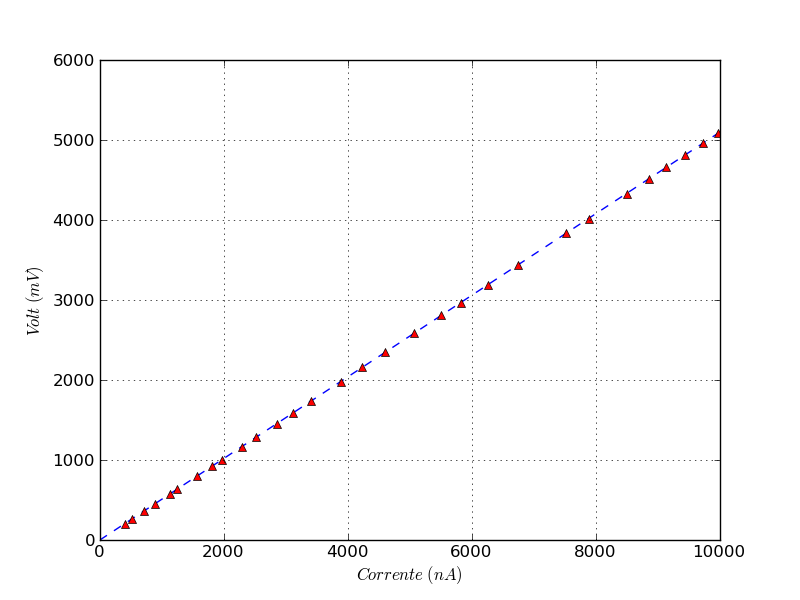
\includegraphics[scale=0.75]{grafici/C1/res1.png}
\
$\chi^2 = 5.76 $

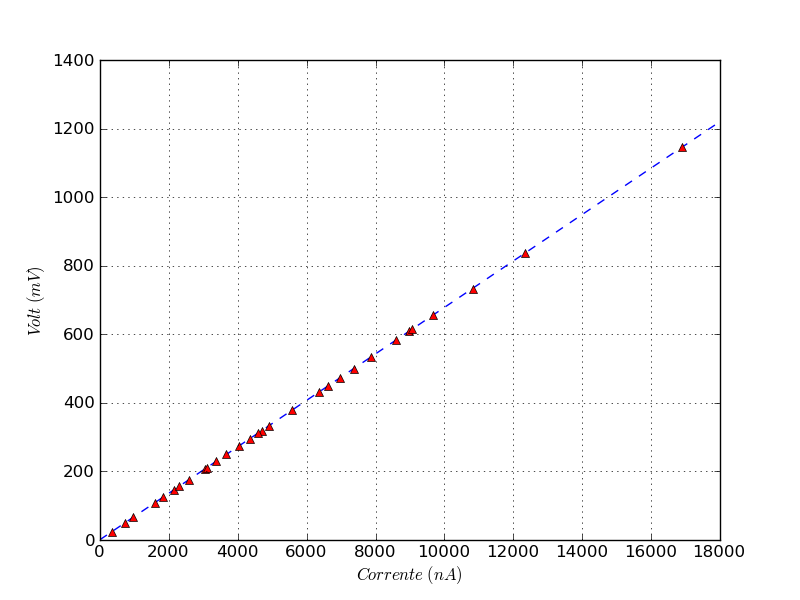
\includegraphics[scale=0.75]{grafici/C1/res2.png}

$\chi^2 = 4.88 $

Misuro la resistenza interna del voltometro, mantenendo costante la ddp a $14.5\ V$ e variando la resistenza all'interno del circuito. 
Il voltmetro è in parallelo al circuito, perciò $R_i$:

$$R_i = \frac{RV}{RI-V} $$

dove R è la resistenza variabile, I la corrente nel circuito e $V= 14.5\ V$

\begin{center}
\begin{tabular}{*{2}{c}}
Resistenza $M\Omega$ & Corrente $nA$\\
\midrule
7&      36\\
9&      32\\
10& 30\\
11&     29\\
12&     28\\
13&     27\\
14&     26\\
15&     26\\
16&     25\\
17&     24\\

\end{tabular}

La resistenza risulta $9.20 \pm 0.27 \ M \Omega$.


Misuriamo la resistenza interna dell'amperometro, che è collegato in serie al circuito. 

$$R_i = \frac{V-RI}{I}$$

In questo caso, R è fissato ($R=0.5 \Omega$) e sono V e I a variare
\begin{tabular}{*{2}{c}}
Volt $mV$ & Corrente $nA$\\
\midrule
22&      1769\\
40&      3271\\
60&      5047\\
105&     8938\\
133&     11201\\
142&     12021\\
164&     13882\\
174&     14745\\
208&     17604\\
232&     19671\\



\end{tabular}

La resistenza interna risulta $11.42 \pm 0.45 \Omega$


\end{center}


Colleghiamo una piccola lampada a filamento al circuito, e verifichiamo che il suo comportamento resistivo non segue la legge di Ohm. 

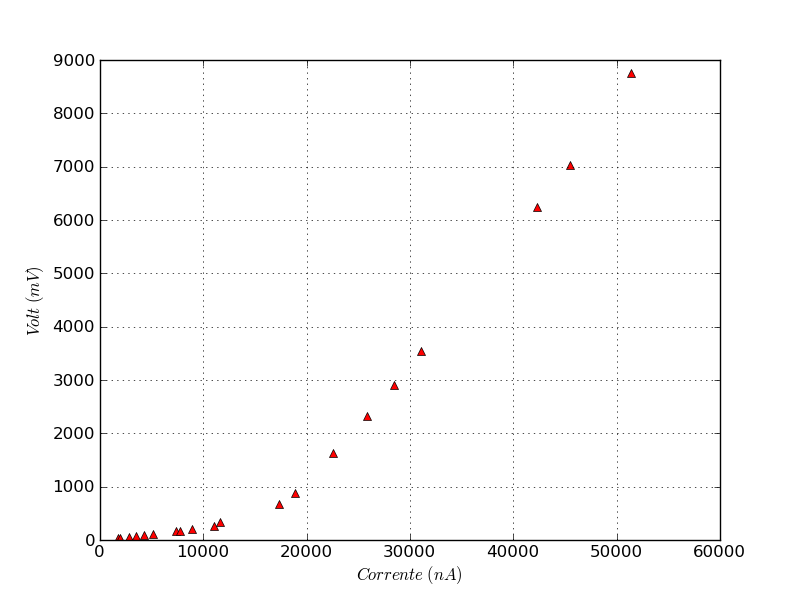
\includegraphics[scale=0.75]{grafici/C1/lampa.png}

La lampadina ha un comportamento non-ohmico nel momento in cui il filamento si scalda sufficientemente e inizia ad emettere luce ($500mV$).


\section{Partitore resistivo}

\subsection{Situazione senza carico}
\begin{center}
\begin{tabular}{*{2}{c}}
$V_{in}$ & $\frac{V_{in}}{V_{out}}$\\
\midrule
329.0 & 0.5015 \\
493.0 & 0.501 \\
544.0 & 0.5018 \\
618.0 & 0.5016 \\
667.0 & 0.5007 \\
776.0 & 0.5 \\
803.0 & 0.5006 \\
927.0 & 0.5005 \\
1078.0 & 0.5 \\
1285.0 & 0.4996 \\
\end{tabular}

\end{center}

$\chi^2=0.0169147373983$


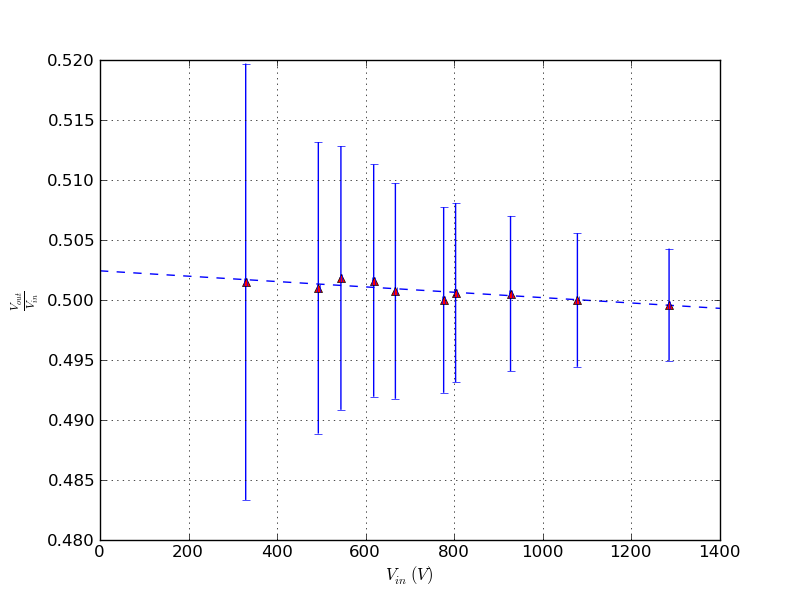
\includegraphics[scale=0.75]{grafici/C1/part1.png}

\subsection{Situazione con carico}
\begin{center}

\begin{tabular}{*{2}{c}}
$V_{in}$ & $\frac{V_{in}}{V_{out}}$\\
\midrule
220.0 & 3.1 \\
276.0 & 3.1051 \\
302.0 & 3.1126 \\
410.0 & 3.1073 \\
511.0 & 3.1115 \\
559.0 & 3.1055 \\
624.0 & 3.109 \\
752.0 & 3.109 \\
906.0 & 3.1093 \\
1036.0 & 3.111 \\
\end{tabular}

\end{center}
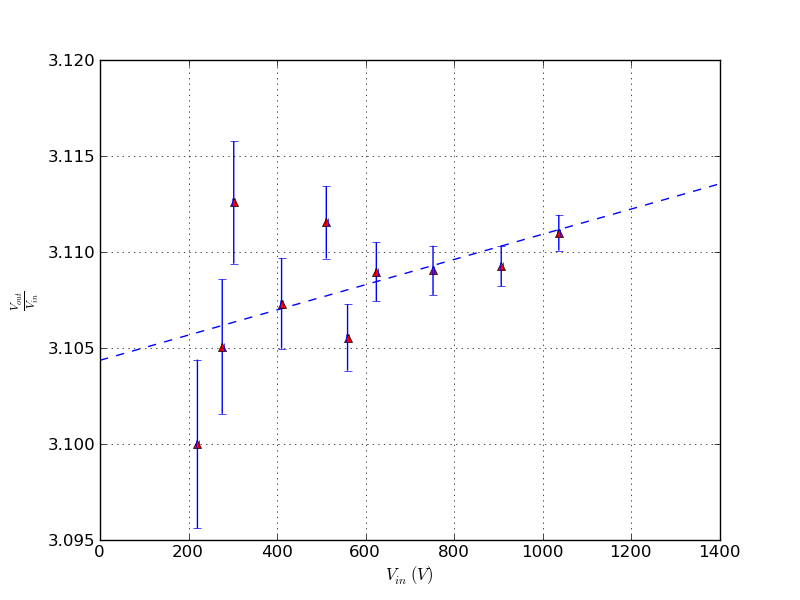
\includegraphics[scale=0.75]{grafici/C1/part2.png}

$\chi^2 = 12.9963702671$

% \begin{sagesilent}
import numpy as np

rc = np.recfromcsv("dati/C2-RC.csv")
rl = np.recfromcsv("dati/C2-RL.csv")


def stampa_dati(wa, header):
  s = r"\begin{tabular}{c*{" + "%d" % (len(wa.dtype)-1)
  s += r"}{|c}}"
  s += "%s \\\\" % (header)
  s += r"\midrule"
  for i in range(0, len(wa)):
    a = ["%s" %x for x in wa[i]]
    s += "%s \\\\" % join(a, "&")
  s += r"\end{tabular}"
  return s
\end{sagesilent}



\chapter{C2}

\section{Risposta in frequenza del multimetro}



\begin{center}
\includegraphics[scale=0.75]{grafici/C2/cv.png} 
\end{center}

Per il grafico in alto,che mostra la lettura dell'intensità di corrente in funzione della frequenza, l'errore è dato dalla sensibilità dello strumento: $\sigma_i = 0.1\ mA$.
\

Il secondo grafico, che mostra i limiti operativi del multimetro rispetto la frequenza, L'errore sulla lettura dal multimetro è la sensibilità dello strumento: $\sigma_{mu} = 0.005\ V$. Per stimare l'errore su $V_{RM}$ abbiamo usato la deviazione standard, assumendo quindi che $V_{RMS}$ dovrebbe rimanere costante. 
Indi per cui, la propagazione degli errori risulta:
$$\sigma_r = \sqrt{\frac{\sigma_{mu}^2}{V_{RMS}^2} + \frac{\sigma_{rms}^2}{V_{RMS}^4}}$$

%E' giusto pensare che rimanga costante?f'

\section{Misura di impedenze ignote}

Scopo di questa seconda parte è misurare l'impedenza di un circuito RC e RL in frequenza alternata. Mostreremo la dipendenza di Z dalla frequenza.


\begin{center}

%\sagestr{stampa_dati(rc, r"Frequenza (Hz) & I (mA) & Valore mu & $V_{rms}$ (V)")}
\end{center}


\begin{center}
\includegraphics[scale=0.75]{grafici/C2/rc.png} 
\end{center}

Dal fit ricavo: $C = 374.53\pm8.44 nF$, che rientra nei valori aspettabili, dato che il valore teorico è $367 nF$. 
Il $chi^{\tilde}^2= 1.4461 $ 

%chi quadro rotto da sistemare.

\begin{center}

%\sagestr{stampa_dati(rl, r"Frequenza (Hz) & I (mA) & Valore mu & $V_{rms}$ (V)")}
\end{center}



\begin{center}
\includegraphics[scale=0.75]{grafici/C2/rl.png} 
\end{center}

$L = 0.016074\pm 0.000092 H$
$\chi^{\tilde}^2 = 1.4546$





% \chapter{C4}

\begin{sagesilent}

import numpy as np
from scipy import odr
import matplotlib.pyplot as plt

trasfm = np.recfromcsv("dati/C4-tensione-fase.csv")

#Sottosmorzamento tempo-volt
#Smorzamento critico tempo-volt
#Sovrasmorzamento tempo-volt
\end{sagesilent}


\begin{sagesilent}

#Funzione di trasferimento del modulo: freq-volt
#RLC in corrente alternata
dati = np.recfromcsv("dati/C4-tensione-fase.csv")
var('x,l,c,v,w')
r = 300
def f(x, l, w, v):
    return (v*2*3.14*x*w)/( sqrt( (2*3.14*x*w)^2+(w*l/r)^2*((2*3.14*x)^2-w^2)^2 ) )
    
puls = dati['frequenza_hz'] #*2*3.14
ennupla = list(((puls[i]), dati['v_out__v_in'][i]) for i in range(0,len(dati['frequenza_hz'])))


fit = find_fit(ennupla, f, parameters=[l,w,v], variables=[x], solution_dict=True)

print fit

plt.clf()
xin = np.arange(100, 100000, 10)
yin = f(xin, fit[l], fit[w], fit[v])
plt.semilogx(xin,yin, 'g--')
plt.semilogx(dati['frequenza_hz'], dati['v_out__v_in'], 'ok')

plt.xlabel(r"$\omega$ [$rad/s$]")
plt.ylabel(r"$V(\omega)$ [$rad$]")
plt.grid(True)

plt.savefig("grafici/C4-ris.png", dpi=300)

#Funzione di trasferimento fase:freq-rad
  
\end{sagesilent}

\includegraphics[scale=0.75]{grafici/C4-ris.png}



%Sottosmorzamento
\begin{sagesilent}
 
om = 2*n(pi)*100
t =np.array([190,570,950,1520])
picchi=np.array([520,-148,60,-24])

def func(P,x):
    return P[0]*P[1]*P[2]*exp(-P[3]*t)*(P[3]*cos(om*x)+om*sin(100*x))

#var('x,r,c,v,g')
#def f(x,r,c, v, g):
#    return r*c*v*exp(-g*t)*(g*cos(om*x)+om*sin(100*x))
    
plt.clf()
plt.plot(t,picchi,'bo')

mod = odr.Model(func)
data = odr.RealData(t,picchi)
done = odr.ODR(data, mod, beta0=[1.,1.,1.,1.],maxit=1000)
sotto = done.run()

#xin = np.arange(min(t),max(t),1)
#yin = func(sotto.beta, xin)

#plt.plot(xin,yin,'g--')
plt.xlabel(r"$\omega$ [$rad/s$]")
plt.ylabel(r"$V(\omega)$ [$rad$]")
plt.savefig("grafici/C4-om.png",dpi=300)
 
\end{sagesilent}

\begin{center}
 \includegraphics[scale=0.75]{grafici/C4-om.png}
\end{center}

%Funzione di trasferimento del modulo
% \begin{sagesilent}
% 
% freq = trasfm['frequenza_hz']
% v = trasfm['v_out_v_in']
% 
% #Funzione di trasferimento del modulo
% 
% def fu(P,x):
%     return (P[0]*2*3.14*x*P[1])/( sqrt( (2*3.14*x*P[1])^2+(w*P[2]/R)^2*((2*3.14*x)^2-[1]^2)^2 ) )
% 
%   
% myodr, chi = fit_chiquad(freq, v, fu, ysigma=yerr, param=[mytransm.beta])
% print "Chi quadro %.4f" % chi
%   
% \end{sagesilent}


% 
\chapter{Interferometro (O2)}

\subsubsection{ strumenti}


\subsubsection{Misura della lunghezza d'onda del laser}

$$ \lambda = \frac{2d}{m} $$

con $d$ spostamento dello specchio mobile e $m$ numero di massimo attraversati (visualizzati sullo schermo).

\begin{center}

\begin{tabular}{c c}
\textbf{Fabry-Perot} & \hspace{2cm} \textbf{Michelson}\\
\\
\begin{tabular}{c|c|c|c|c|c}
d ($\mu m$)& $\sigma_d$ & m & $\sigma_m$ & $\lambda$ ($nm$) & $\sigma_{\lambda}$\\
\midrule
29 & 1 & 87 & 4 & 670 & 38\\
25 & 1 & 79 & 1 & 632 & 26\\
31 & 1 & 81 & 1 & 642 & 26\\
26 & 1 & 75 & 7 & 693 & 70\\
20 & 1 & 64 & 5 & 625 & 58\\
35 & 1 & 107 & 5 & 654 & 36\\


?? \\

\end{tabular}

& \hspace{2cm}

\begin{tabular}{c|c|c|c|c|c}
d ($\mu m$) & $\sigma_d$ & m & $\sigma_m$ & $\lambda$ ($nm$) & $\sigma_{\lambda}$\\
\midrule
25 & 1& 75 & 2 & 666 & ?\\
75 & 1& 72 & 1 & 697 & ?\\

\end{tabular}

\end{tabular}

\end{center} 

In cui $\sigma_{\lambda}$ è data dalla propagazione dell'errore su d e m:

$$ \sigma_{\lambda} = \sqrt{ ( \frac{\partial \lambda}{\partial d} \sigma_{d} )^2 + ( \frac{\partial \lambda}{\partial m} \sigma_{m} )^2 } $$

Valore atteso: 632.8 $nm$\\

Dalla media pesata con errore otteniamo una $\lambda$ media di:

$$ \lambda =\displaystyle \sum_i{\frac{\frac{x_i}{(\sigma_i)^2}}{\frac{1}{(\sigma_i)^2}}} \pm \displaystyle\sum_i{\frac{1}{(\sigma_i)^2}} = 644 \pm 14 nm $$

\subsection{Misura dell'indice di rifrazione dell'aria}

Si pone una cella a vuoto (spessore $d=3 cm$) tra lo specchio semi-riflettente e lo specchio rotante (che in questa parte dell'esperienza rimane fisso) nell'interferometro di Michelson. La cella è collegata ad un compressore, e un barometro segna la variazione di pressione.
Raccogliamo il numero di massimi che attraversano lo schermo al variare della pressione e ricaviamo $n_{aria}$ dalla relazione:
$$ n = mP+1 $$
$$ m = \frac{n_i - n_f}{P_i-P_f} = \frac{N \lambda_0}{2d(P_i-P_f)}$$

\begin{center}
\begin{tabular}{c|c|c}
$P_i-P_f$ ($kPa$) & N & m \\
\midrule
70 & 19 & $2.859\cdot10^{-6}$\\
\end{tabular}
\end{center}

$$ n = mP+1 = 1.000289 \pm \text{booh, di quanto sono le incertezze?}$$

Valore atteso: 1.000293

\subsection{Misura dell'indice di rifrazione del vetro}

In modo analogo a quanto fatto per la misura di $n_{aria}$, si pone tra lo specchio semi-riflettente e lo specchio rotante una lastra di vetro (spessore $t= 5 mm$). Raccogliamo il numero N di frange di interferenza contate per uno spostamento angolare superiore a $10°$, e ricaviamo $n_{vetro}$ dalla relazione:

$$n=\frac{(2t-N\lambda_0)(1-cos(\theta))}{2t(1-cos\theta)-N\lambda_0}$$

Per fissare lo zero, troviamo l'angolo di deviazione minima.

$\delta = 0.6 \pm (?) $

\begin{center}
\begin{tabular}{c|c|c|c|c|c}
$\theta (°) $ & $\sigma_{\theta}$ & N & $\sigma_{N}$ & n & $\sigma_{n}$\\
\midrule
10.8 & 3 & 112 & 3 & 1.578 & ? \\
9.2 & 3 & 87 & 2 & 1.529 & ? \\
\end{tabular}
\end{center}

\subsection{Reticolo ad incidenza radente}

\begin{sagesilent}

import numpy as np
import matplotlib.mlab as ml

dati = np.recfromcsv("dati/interferometro.csv")

var('d, h, l, k,n, sigma_h, sigma_l,sigma_k')
lamb(h,k,l) = (d/n)*(cos(atan(h/l))-cos(atan(k/l)))


elle = 344

dif = lamb.differentiate()
errs = vector([sigma_h, sigma_k, sigma_l])
slam = vector([d, h, l])

for i in range(0, len(dif)):
    slam[i] = (dif[i]*errs[i])
    
errscal = abs(slam)
\end{sagesilent}


In questa parte dell'esperienza misuriamo la $\lambda$ della luce a laser attraverso considerazioni geometriche riguardo ai fenomeni di interferenza e riflessione. Infatti, noto il passo del reticolo (nel nostro caso il reticolo consiste in un righello metallico, e dunque il passo è $d = 1 mm$), possiamo ricavare $\lambda$ dalla relazione:

$$ n\lambda = d(cos\theta_i-cos\theta_r) $$

con $l = 344 cm $ (distanza sorgente-schermo) e $\theta = arctg\frac{h}{l}$

Per considerare l'errore che commettiamo su $l$, dunque, la funzione che ci interessa è:
$$\lambda\sage{lamb}$$
Il cui differenziale è:
$$\nabla \lambda \sage{dif}$$

Dunque, l'incertezza su $\lambda$ è data dalla relazione
$$\sigma_\lambda = \sage{errscal}$$

\begin{sagesilent}
subd = errscal.subs(d=0.1,h=30,l=elle,sigma_h=0.3,sigma_k=0.3,sigma_l=3)
sublambda = lamb.subs(d=0.1,h=30,l=elle)

lambdas = [abs((sublambda.subs(h=int(dato['h']), k=dato['k'], n=int(dato['n']))*10^7)).n(digits=4) for dato in dati]
errorsarr = np.array([(subd.subs(n=int(dato['n']), k=dato['k'])*10^7).n(digits=4) for dato in dati], dtype='f4')
print errorsarr

dati = ml.rec_append_fields(dati, "lambda", lambdas)
dati = ml.rec_append_fields(dati, "sigma_lambda", errorsarr)

meanlambda = np.average(dati['lambda'], weights=1./(dati['sigma_lambda']**2))
errtot = 1/sum(1/dati['sigma_lambda']**2)

def stampa_dati(wa, header):
  s = r"\begin{tabular}{c*{" + "%d" % (len(wa.dtype)+1)
  s += r"}{|c}}"
  s += "%s \\\\" % (header)
  s += r"\midrule"
  for i in range(0, len(wa)):
    a = ["%.4G" % x for x in wa[i]]
    s += "%s \\\\" % join(a, "&")
  s += r"\end{tabular}"
  return s
\end{sagesilent}

Sostituendo:
\begin{center}
\sagestr{stampa_dati(dati, "n & k (cm) &h (cm)& $\lambda$ (nm) & $\sigma_\lambda$ ")}
\end{center}
Graficati:
\begin{sagesilent}
import matplotlib.pyplot as plt
plt.clf()
plt.errorbar(dati['k'], dati['lambda'], dati['sigma_lambda'], fmt="ro")
plt.grid(True)
plt.ylabel(r"$\lambda$ (nm)")
plt.xlabel("k (cm)")
plt.savefig("grafici/interfer-lambda-con-err.png", dpi=300)
\end{sagesilent}

\includegraphics[scale=0.75]{grafici/interfer-lambda-con-err.png}

Valor medio: $\sage{int(meanlambda)}\pm\sage{int(errtot)}$ nm

% \begin{sagesilent}
import matplotlib.pyplot as plt
import numpy as np
import scipy.optimize as opt
\end{sagesilent}


\chapter{Microonde}

\section{Riflessione}

Intendiamo verificare la legge di Cartesio utillizando una lastra di metallo come superficie rifelttente, posizionandola su un supporto magnetico sul goniometro.

\begin{equation}
sin(\theta_{incidente}) = sin(\theta_{rifratto})
\end{equation}

\begin{sagesilent}
dati = np.recfromcsv('dati/MICROONDE/cartesio.csv')
\end{sagesilent}

\begin{center}
\sagestr{stampa_dati(dati, r'$\theta_{inc}$ (rad) & $\theta_{rif}$ (rad) ' )}
\end{center}


\section{Misura della lunghezza d'onda}

\begin{sagesilent}
dati = np.recfromcsv('dati/MICROONDE/lambda.csv')

#Calcolo lambda:

d = np.array(dati['distanza'])
d.astype(float)
n = np.array(dati['enne'])
n.astype(float)
lam = 2*d/n
sigmad = 0.5
errlam = 2/n*sigmad

lmedia = np.average(lam)
confronto = abs(2.85-lmedia)

dati = ml.rec_append_fields(dati, 'lungonda', lam)

\end{sagesilent}

Se si pongono trasmettitore e ricevitore ad una distanza di $\frac{n \lambda}{2}$, si può osservare che essi generano onde stazionarie. Infatti le antenne delle due apparecchiature riflettono parzialmente le onde che ricevono, e se li si mette in una condizione tale per cui le onde riflesse hanno la stessa fase delle onde incidenti si osservano dei massimi, viceversa, se le fasi sono antagoniste, si avrà una condizione di nodo.
Ricaviamo la lunghezza d'onda posizionando emettitore e ricevitore ai capi del metro, e muovendo il ricevitore lungo questo osserviamo  il passaggio alterno per massimi e minimi di intensità. Ricaviamo $\lambda$ dalla nota formula per le onde stazionarie:
\begin{equation}
d = n\frac{\lambda}{2}
\label{d}
\end{equation}


\begin{center}
\sagestr{stampa_dati(dati, r'$d$ (cm) & $n$ (rad) & $\lambda$ (cm)' )}
\end{center}

Otteniamo una lambda media: $$ \sage{lmedia} \pm \sage{errlam}$$

%Dal confronto con la $\lambda$ (2.85 cm) teorica otteniamo: $\lambda_{teo} - \lambda_{cal} || = \sage{confronto} < 2 \sigma ( = 2 \sage{errlam} $


\section{Rifrazione attraverso un prisma}

In questa parte dell'esperienza si verifica la legge di snell:
\begin{equation}
\frac{sin(\theta_{i})}{sin(\theta_{r})} = \frac{n_2}{n_1}
\end{equation}
A tal fine posizioniamo una pedana di polistirolo sul goniometro, e vi poniamo sopra un prisma, sempre di polistirolo, contenente "styrene pellets". Si verifica la legge per vari massimi di intensità (Nota: $n_1$ = 1).

%Dati???

\section{Polarizzazione}

\begin{sagesilent}
#Calcolo dell'intensità con la legge di Malus

dati = np.recfromcsv('dati/MICROONDE/malus.csv')

izero = 8.75
gamma=dati['gamma']*3.14/180
iteorico = izero*(cos(gamma))**2

dati = ml.rec_append_fields(dati, 'iteo', iteorico)

\end{sagesilent}


Le microonde uscenti dal trasmettitore sono polarizzate linearmente, per cui soddisfano alla legge di Malus che lega l'intensità all'angolo tra la normale al ricevitore e la direzione dell'onda. Fissata una distanza, posizioniamo emettitore e ricevitore uno difronte all'altro e misuriamo la diminuzione d'intensità relativa al variare dell'angolo rispetto all'orizzontale di emettitore-ricevitore. Di seguito i dati letti sul multimetro a confronto con l'intensità teorica data dalla legge di Malus:

\begin{equation}
I = I_{0} cos^2 \gamma
\end{equation}

\begin{center}
%\sagestr{stampa_dati(dati, r'$I$ (Volt) & $\gamma$ (rad) & $I_{teorico}$ (Volt) ' )}
\end{center}


\section{Interferenza da doppia fenditura}
\begin{sagesilent}
dfen = np.recfromcsv("dati/microonde-doppiafen.csv")
dfen.sort()
var('x,a,w,t')
model(x, a, w, t) = a*sin(w*x+t)

def ff(x, a,w,t):
  f = fast_callable(model)
  return f(x,a,w,t)

#print dfen['angolo']
pars, pcov = opt.curve_fit(ff, np.array(dfen['angolo']), np.array(dfen['volt']), p0=[500., 50., 1.])

print pcov

print pars
plt.clf()
xin = np.arange(min(dfen['angolo']), 220, 1)
print "now"
yin = ff(xin, pars[0], pars[1], pars[2])
plt.plot(xin, yin)
plt.plot(dfen['angolo'], dfen['volt'], 'o--')

plt.savefig("grafici/microonde-doppiafend.png")
\end{sagesilent}


Utilizzando un supporto magnetico sul goniometro, montiamo tre lastre di metallo in modo da avere due
fenditure di circa 1,5 cm. Spostando il ricevitore si troviamo i massimi e i minimi di interferenza al fine di verificare la
loro posizione rispetto alla previsione teorica: $d \sin(\theta) = n \lambda$ (per i massimi, con d distanza delle fenditure, $\theta$ angolo
rispetto alla perpendicolare, n numero intero).

\includegraphics[scale=0.75]{grafici/microonde-doppiafend.png}

\section{Specchio di Lloyd}

\begin{sagesilent}
#Calcolo della lunghezza d'onda

dati = np.recfromcsv('dati/MICROONDE/lloyd.csv')

d = dati['delta']
enne = dati['n']

lam = 2*d/enne


dati = ml.rec_append_fields(dati, 'lung_onda', lam)

\end{sagesilent}

Posizioniamo emettitore e ricevitore a distanza di un circa un metro, uno dinnanzi all'altro. Su un secondo metro, perpendicolare alla direzione emettitore-ricevitore e passante per il goniometro, montiamo una lastra di metallo che funge da specchio: in tal modo generiamo un'interferenza dovuta alla differenza di cammino delle onde (una parte arriva direttamente al ricevitore, mentre altre onde percorrono il cammino dall'emettitore allo specchio e dallo specchio al ricevitore). Cerchiamo il minimo di intensità con lo specchio a distanza minima dal goniometro e raccogliamo i massimi di intensità al variare della distanza, per determinare $\lambda$ come in \ref{d}

\begin{center}
%\sagestr{stampa_dati(dati, r'$d$ (cm) & $n$ & $\lambda$ ' )}
\end{center}

\section{Diffrazione di Bragg}

\begin{sagesilent}
#Grafico dell'intensità in funzione dei gradi

dati = np.recfromcsv('dati/MICROONDE/bragg.csv')
plt.clf()
plt.plot(dati['theta'], dati['volt'],'ro')

plt.savefig("grafici/microonde-bragg.png")

\end{sagesilent}


Nell'ultima parte dell'esperimento ci proponiamo di verificare la legge di Bragg, 
\begin{equation}
n \lambda = 2 d \sin(\theta)
\end{equation}
la quale esprime analiticamente i fenomeni di interferenza causati dalla riflessione di onde su piani paralleli di un reticolo cristallino. Per riprodurre il fenomeno, facciamo incidere le microonde su un cubo di polistirolo su cui sono inserite su spaziature regolari delle sferette di acciaio.

Nella formula:\\
$\theta$ è l'angolo che il fascio incidente forma col piano cristallino\\
$\lambda$ è la lunghezza d'onda della radiazione\\
$d$ è la distanza tra due piani adiacenti\\
$n$ indica l'ordine della diffrazione (tipicamente solo quello per n=1 è apprezzabile).\\

La formula si spiega in maniera analitica considerando una differenza di cammino ottico pari a $2d\sin(\theta)$.


\includegraphics[scale=0.75]{grafici/microonde-bragg.png}

\section{Analisi dati}

\section{Allegato: dati}
\begin{sagesilent}
def stampa_dati(wa, header):
  s = r"\begin{tabular}{c*{" + "%d" % (len(wa.dtype)-1)
  s += r"}{|c}}"
  s += "%s \\\\" % (header)
  s += r"\midrule"
  for i in range(0, len(wa)):
    a = ["%s" %x for x in d[i]]
    s += "%s \\\\" % join(a, "&")
  s += r"\end{tabular}"
  return s
\end{sagesilent}

\begin{center}

% \sagestr{stampa_dati(d, r"Frequenza (Hz) & I (mA) & Valore mu & $V_{rms}$ (V)")}
\end{center}


%INIZIALIZZAZIONE e LIBRERIE
\begin{sagesilent}
#Importo librerie necessarie
import numpy as np
from scipy import odr
import matplotlib.pyplot as plt
import matplotlib.mlab as ml

#classica funzione chiquadrato, non cancellare
def chiquad(xdata, ydata, yfunc, ysigma = (), param=()):
    yteo = yfunc(xdata, *param)
    ddof = len(xdata) - 1 - len(param)
    if (np.isscalar(ysigma)):
        ys = np.ones_like(xdata)*ysigma
    else:
        ys = ysigma
 
    if (len(ys)):
        return sum(((ydata-yteo)/ys)**2)
    else:
        return sum((ydata-yteo)**2/yteo)

        
#Funzione stampadati
def stampa_dati(datiarr, header):
  s = r"\begin{tabular}{c*{" + "%d" % (len(datiarr.dtype)-1)
  s += r"}{|c}}"
  s += "%s \\\\" % (header)
  s += r"\midrule"
  for i in range(0, len(datiarr)):
    a = ["%.3G" %x for x in datiarr[i]]
    s += "%s \\\\" % join(a, "&")
  s += r"\end{tabular}"
  return s
        
\end{sagesilent}



\chapter{ Spettrometro (O3)}


\section*{Reticolo}

\subparagraph{Introduzione}

Nella prima parte dell'esperienza misuriamo le lunghezze d'onda corrispondenti a differenti righe spettrali emesse da una sorgente di gas eccitato, attraverso l'uso di un reticolo a diffrazione. \\
Il reticolo a diffrazione consiste in una lastra di vetro su cui sono tracciate delle linee parallele molto sottili. La distanza tra le fenditure dà il passo del reticolo.\\
La luce proveniente dalla sorgente viene fatta passare prima attraverso una fenditura, e successivamente attraverso una lente convergente, il cui piano focale coincide proprio con il piano su cui giace la fenditura: tale sistema prende il nome di collimatore. I raggi paralleli uscenti dalla lente intercettano il reticolo, che attraverso una procedura sperimentale viene posto ortogonalmente al fascio, e da lì vengono deviati di un angolo $\theta$. Un telescopio montato su un piatto rotante permette di osservare le righe d'emissione del gas, ruotando opportunamente la piattaforma secondo la direzione $\theta_{\lambda} $ data dalla legge:
\begin{equation}
sin \theta_{\lambda} = m \frac{\lambda}{d}
\label{eq:theta}
\end{equation}


Da tale legge, dunque possiamo risalire alla lunghezza d'onda, attraverso la lettura dell'angolo di cui si è ruotato il telescopio (la piattaforma è dotata di un goniometro).

\subparagraph{Passo del reticolo}

Prima di iniziare la raccolta dati è necessario posizionare il reticolo in modo tale che risulti perpendicolare al fascio di luce incidente. A tal fine misuriamo gli angoli di deviazione per massimi dello stesso ordine, e lo zero corrisponde alla direzione della luce non deviata. Otteniamo $\theta_{0} = 283 3' $ \\
Per stabilire il passo del reticolo utilizziamo una sorgente di cui è nota la lunghezza d'onda (lampada a sodio: $\lambda_{Na} = 589.3 $ nm ), e giriamo la \ref{eq:theta} per ricavare d. In particolare utilizziamo una versione della \ref{eq:theta} che diminuisca l'errore sperimentale a cui sono soggette le misure, in cui a $\theta$ si sostituisce la media dei due angoli destro e sinistro $\theta_{dx} $ e $\theta_{sx}$.

\begin{equation}
d = \frac{n \lambda}{sin(\frac{\theta_{dx}-\theta_{sx}}{2})}
\end{equation}

L'errore su d si ottiene dalla propagazione degli errori associati alla misura degli angoli. Si ha dunque:

\begin{sagesilent}


dati = np.recfromcsv('dati/spettro-reticolo.csv')
var('n')
var('dtheta', latex_name=r'\Delta\theta')
var('lam', latex_name=r'\lambda')
var('sigma_dtheta', latex_name=r'\sigma_{\Delta\theta}')
d(dtheta)=n*lam/(sin(dtheta))
derror = (d.diff())*sigma_dtheta
sigmadth=2*0.0087

dfasterror = fast_float(derror)
#print derror.subs(lam=1,n=2,dtheta=1.).n()

# dati['deltatheta'] = dati['deltatheta']*10^(-3)

def ret_error(dato):
  deltheta = dato['deltatheta']
  res = derror(dtheta=deltheta).subs(lam=dato['lambda']*10^-9, n=int(dato['n']),
                    sigma_dtheta=sigmadth)
  return abs(res[0])
  
errorsarr = np.array([ret_error(dato) for dato in dati ])

dcalc = np.array([float(d.subs(lam=dato['lambda']*10^-9,n=int(dato['n']),dtheta=dato['deltatheta']).n(digits=2) ) for dato in dati ])
dati = ml.rec_append_fields(dati, "d", dcalc*10^6)
dati = ml.rec_append_fields(dati, "error_d", errorsarr*10^6)

\end{sagesilent}
$$d:\sage{d}$$
Derivata e moltiplicata per $\sigma_{\Delta\theta}$, otteniamo $\sigma_d$:
$$\sigma_d: \sage{derror}$$
Per i nostri dati:
\begin{center}
\sagestr{stampa_dati(dati, r'n & $\lambda$ (nm) & $\Delta\theta$ (rad) & d ($\mu$m)& $\sigma_d$ ($\mu$m)' )} 
\end{center}

\begin{sagesilent}
media = np.average(dati['d'], weights=1./dati['error_d']**2)
errmedia = 1./np.sqrt(sum(1./dati['error_d']**2))
\end{sagesilent}

Otteniamo $d=\sage{round(media, 3)}\pm\sage{errmedia.n(digits=2)}$ $\mu$m.




\section*{Prisma}


Nella seconda parte dell'esperienza intendiamo verificare la legge di Cauchy:
\begin{equation}
n = a + \frac{b}{\lambda^2}
\label{Cauchy}
\end{equation}
che lega l'indice di rifrazione di un materiale alla lunghezza d'onda della luce incidente, nel caso dell'indice di rifrazione di un prisma di vetro.
I coefficienti a e b che figurano in \ref{Cauchy} vengono determinati con il metodo dei minimi quadrati. \\
Pertanto misuriamo n corrispondente alle differenti righe spettrali del mercurio (utilizziamo una lampada Hg come sorgente) attraverso la legge:
\begin{equation}
n = \frac{sin(\frac{\alpha + \delta}{2})}{sin(\frac{\alpha}{2})}
\label{n}
\end{equation}
in cui $\alpha$ è l'angolo al vertice del prisma, di $60°$, e $\delta$ l'angolo di deviazione minima. Nota: al denominatore del membro di destra si è trascurato di mettere $n_{aria}=1$.

Con tale procedura otteniamo i seguenti valori per i parametri:


\begin{sagesilent}
 #Fit per ricavare i parametri della relazione di Cauchy


dati = np.recfromcsv('dati/spettro-cauchy.csv')

l = 1./(dati['l']**2)
n = dati['n']

var('x,P')

#Questa funzione serve solo al chiquadro e per il grafico
def fun(x,a,b):
    return a*x+b


#Questa funzione serve per il fit fatto da odr
def func(P,x):
    return P[0]*x+P[1]
    
mymodel = odr.Model(func)

mydata = odr.RealData(l,n)

myodr = odr.ODR(mydata, mymodel, beta0=[1.,1.],  maxit=5000)
myout = myodr.run()

a = myout.beta[0]
b = myout.beta[1]
chiquadrato = chiquad(np.array(l), n, fun, ysigma=float(0.05), param=[a,b]) 

   
plt.clf()
plt.plot(l,n,'ro')
xin = np.arange(0.9*min(l),1.3*max(l),2*max(l)/10) 
yin = fun(xin,myout.beta[0],myout.beta[1])
plt.plot(xin,yin,'--')
plt.grid(True,which="both")
plt.savefig("grafici/spettro-cauchy.png", dpi=300)
 

\end{sagesilent}


$$a = \sage{myout.beta[1]} \pm \sage{myout.sd_beta[1]}$$
$$b = \sage{myout.beta[0]} \pm \sage{myout.sd_beta[0]}$$
$$ \chi^ 2 = \sage{chiquadrato}$$

Dati raccolti:


\begin{sagesilent}
import numpy as np
import matplotlib.mlab as ml

dati = np.recfromcsv('dati/spettro-cauchy.csv')

var('n, alpha')
var('delta', latex_name=r'\delta')
var('sigma_delta', latex_name=r'\sigma_{\delta}')

d(delta)=sin((alpha+delta)/2)/sin(alpha/2)

derror = (d.diff())*sigma_delta
sigmadel=0.0087
alpha_nostro=1.047


def ret_error(dato):
  res = derror(delta=dato['delta']).subs(alpha=alpha_nostro, n=int(dato['n']),
                    sigma_delta=sigmadel)
  return abs(res[0])
  
errorsarr = np.array([ret_error(dato) for dato in dati ])

dcalc = np.array([float(d(delta=dato['delta']).subs(alpha=alpha_nostro, n=int(dato['n'])).n(digits=2) ) for dato in dati ])

print dati
print dcalc
print errorsarr
dati = ml.rec_append_fields(dati, "error_d", errorsarr)

def stampa_dati(datiarr, header):
  s = r"\begin{tabular}{c*{" + "%d" % (len(datiarr.dtype)-1)
  s += r"}{|c}}"
  s += "%s \\\\" % (header)
  s += r"\midrule"
  for i in range(0, len(datiarr)):
    a = ["%.3G" %x for x in datiarr[i]]
    s += "%s \\\\" % join(a, "&")
  s += r"\end{tabular}"
  return s
\end{sagesilent}

\begin{center}
\sagestr{stampa_dati(dati, r"$\lambda$ (nm) & $n$ & $\delta$ & $\sigma_n$")}
\end{center}


In cui l'errore su $n$ è dato dall'errore su $\delta = 0.0087 rad $ tramite la:

$$\sigma_n: \sage{derror}$$



\begin{center}
\includegraphics[scale=0.75]{grafici/spettro-cauchy.png}
\end{center}




\section*{Determinazionedi una sorgente ignota}
Infine utilizziamo i procedimenti e i valori stimati nelle prime parti dell'esperienza  per determinare, mediante lo spettro, il gas corripondente alla sorgente ignota.\\

Calcoliamo n dalla \ref{n}, ed utilizziamo tali valori per ricavare le lunghezze d'onda dalla \ref{Cauchy}, dove adesso sono noti i parametri a e b:
\begin{equation}
\lambda = \sqrt{\frac{b}{n-a}}
\end{equation}


%Elaborazione dati:


\begin{sagesilent}


dati = np.recfromcsv('dati/spettro-neon.csv')

var('alpha')
var('delta', latex_name=r'\delta')
var('sigma_delta', latex_name=r'\sigma_{\delta}')


n(delta) = sin((alpha+delta)/2)/sin(alpha/2)

nerror = (n.diff())*sigma_delta
sigmadel=0.0087
alpha_nostro=1.047
coeff1=9333.5
coeff2=1.5919
sigma_a = 0.000766
sigma_b = 164.4


def ret_error(dato):
  res = nerror(delta=dato['delta']).subs(alpha=alpha_nostro, sigma_delta=sigmadel)
  return abs(res[0])
  
errorsarr = np.array([ret_error(dato) for dato in dati ])

ncalc = np.array([float(n(delta=dato['delta']).subs(alpha=alpha_nostro).n(digits=2) ) for dato in dati ])

#Determinazione delle lambda incongite

var('a', 'b', 'enne')

l(enne)=sqrt(b/(enne-a))

lcalc= np.array([float(l(enne=dato,digits=4).subs(b=coeff1, a=coeff2)  ) for dato in ncalc ])

#Propagazione errori

#var('sigma_a', 'sigma_b')

#lerror(a,b)=sqrt(b/(enne-a))

#dif = lerror.differentiate()

#dif=vector([lerror.diff(a), lerror.diff(b)])

#def errscal(dato):
 # errs = vector([sigma_a, sigma_b])
 # slam = vector([0, 0])
 # diffVal = dif(a=coeff1, b=coeff2, digits=4).subs(enne=dato)
  
 # for i in range(0, len(dif)):
 #     slam[i] = (diffVal[i]*errs[i])
    
 # return abs(slam)

#print 'ncalc', ncalc

#errorl = np.array([float(errscal(trick) ) for trick in ncalc ])



print dati
print ncalc
print errorsarr
print lcalc
#print errorl
dati = ml.rec_append_fields(dati, "n", ncalc)
dati = ml.rec_append_fields(dati, "error_n", errorsarr)
dati = ml.rec_append_fields(dati, "l", lcalc)
#dati = ml.rec_append_fields(dati, "error_l", errorl)

def stampa_dati(datiarr, header):
  s = r"\begin{tabular}{c*{" + "%d" % (len(datiarr.dtype)-1)
  s += r"}{|c}}"
  s += "%s \\\\" % (header)
  s += r"\midrule"
  for i in range(0, len(datiarr)):
    a = ["%.3G" %x for x in datiarr[i]]
    s += "%s \\\\" % join(a, "&")
  s += r"\end{tabular}"
  return s
\end{sagesilent}

\begin{center}
\sagestr{stampa_dati(dati, r"  $\delta$ & $n$ & $\sigma_n$ & $\lambda$  ") }
\end{center}


% \chapter{Misura della velocità della luce}

L'obiettivo del nostro esperimento è misurare la velocità della luce $c$.

L'apparato di misurazione consiste principalmente in:
\begin{itemize}
 \item Un laser Elio-Neon ($\lambda=32$ nm).
 \item Uno specchio rotante a velocità angolare regolabile.
 \item Due lenti convergenti, di lunghezza focale $l_1 = 48mm$ e $l_2 = 252 mm$.
 \item Un microscopio con beam splitter e micrometro.
\end{itemize}

Lo specchio rotante viene fatto girare con velocità angolare $\omega_1$ in senso orario e $\omega_2$ in senso antiorario. Queste velocità angolari sono identiche nella maggior parte dei casi, e la loro differenza è trascurabile.

Chiamando $s_{cw}$ e $s_{ccw}$ rispettivamente le misure con specchio rotante in senso orario e antiorario, per come è orientata la strumentazione il numero
$$\Delta s = s_{cw} - s_{ccw}$$
deve essere positivo.

Purtroppo però non è questo il caso per qualche misura presa in mattinata, per ragioni sconosciute e che non siamo riusciti a riprodurre. Questi dati sono esclusi dalla misurazione in quanto evidenti errori, e sono mostrati in rosso nel grafico seguente
I dati sono molti, dunque forniamo qui soltanto una visione grafica, e lasciamo la tabella come allegato.

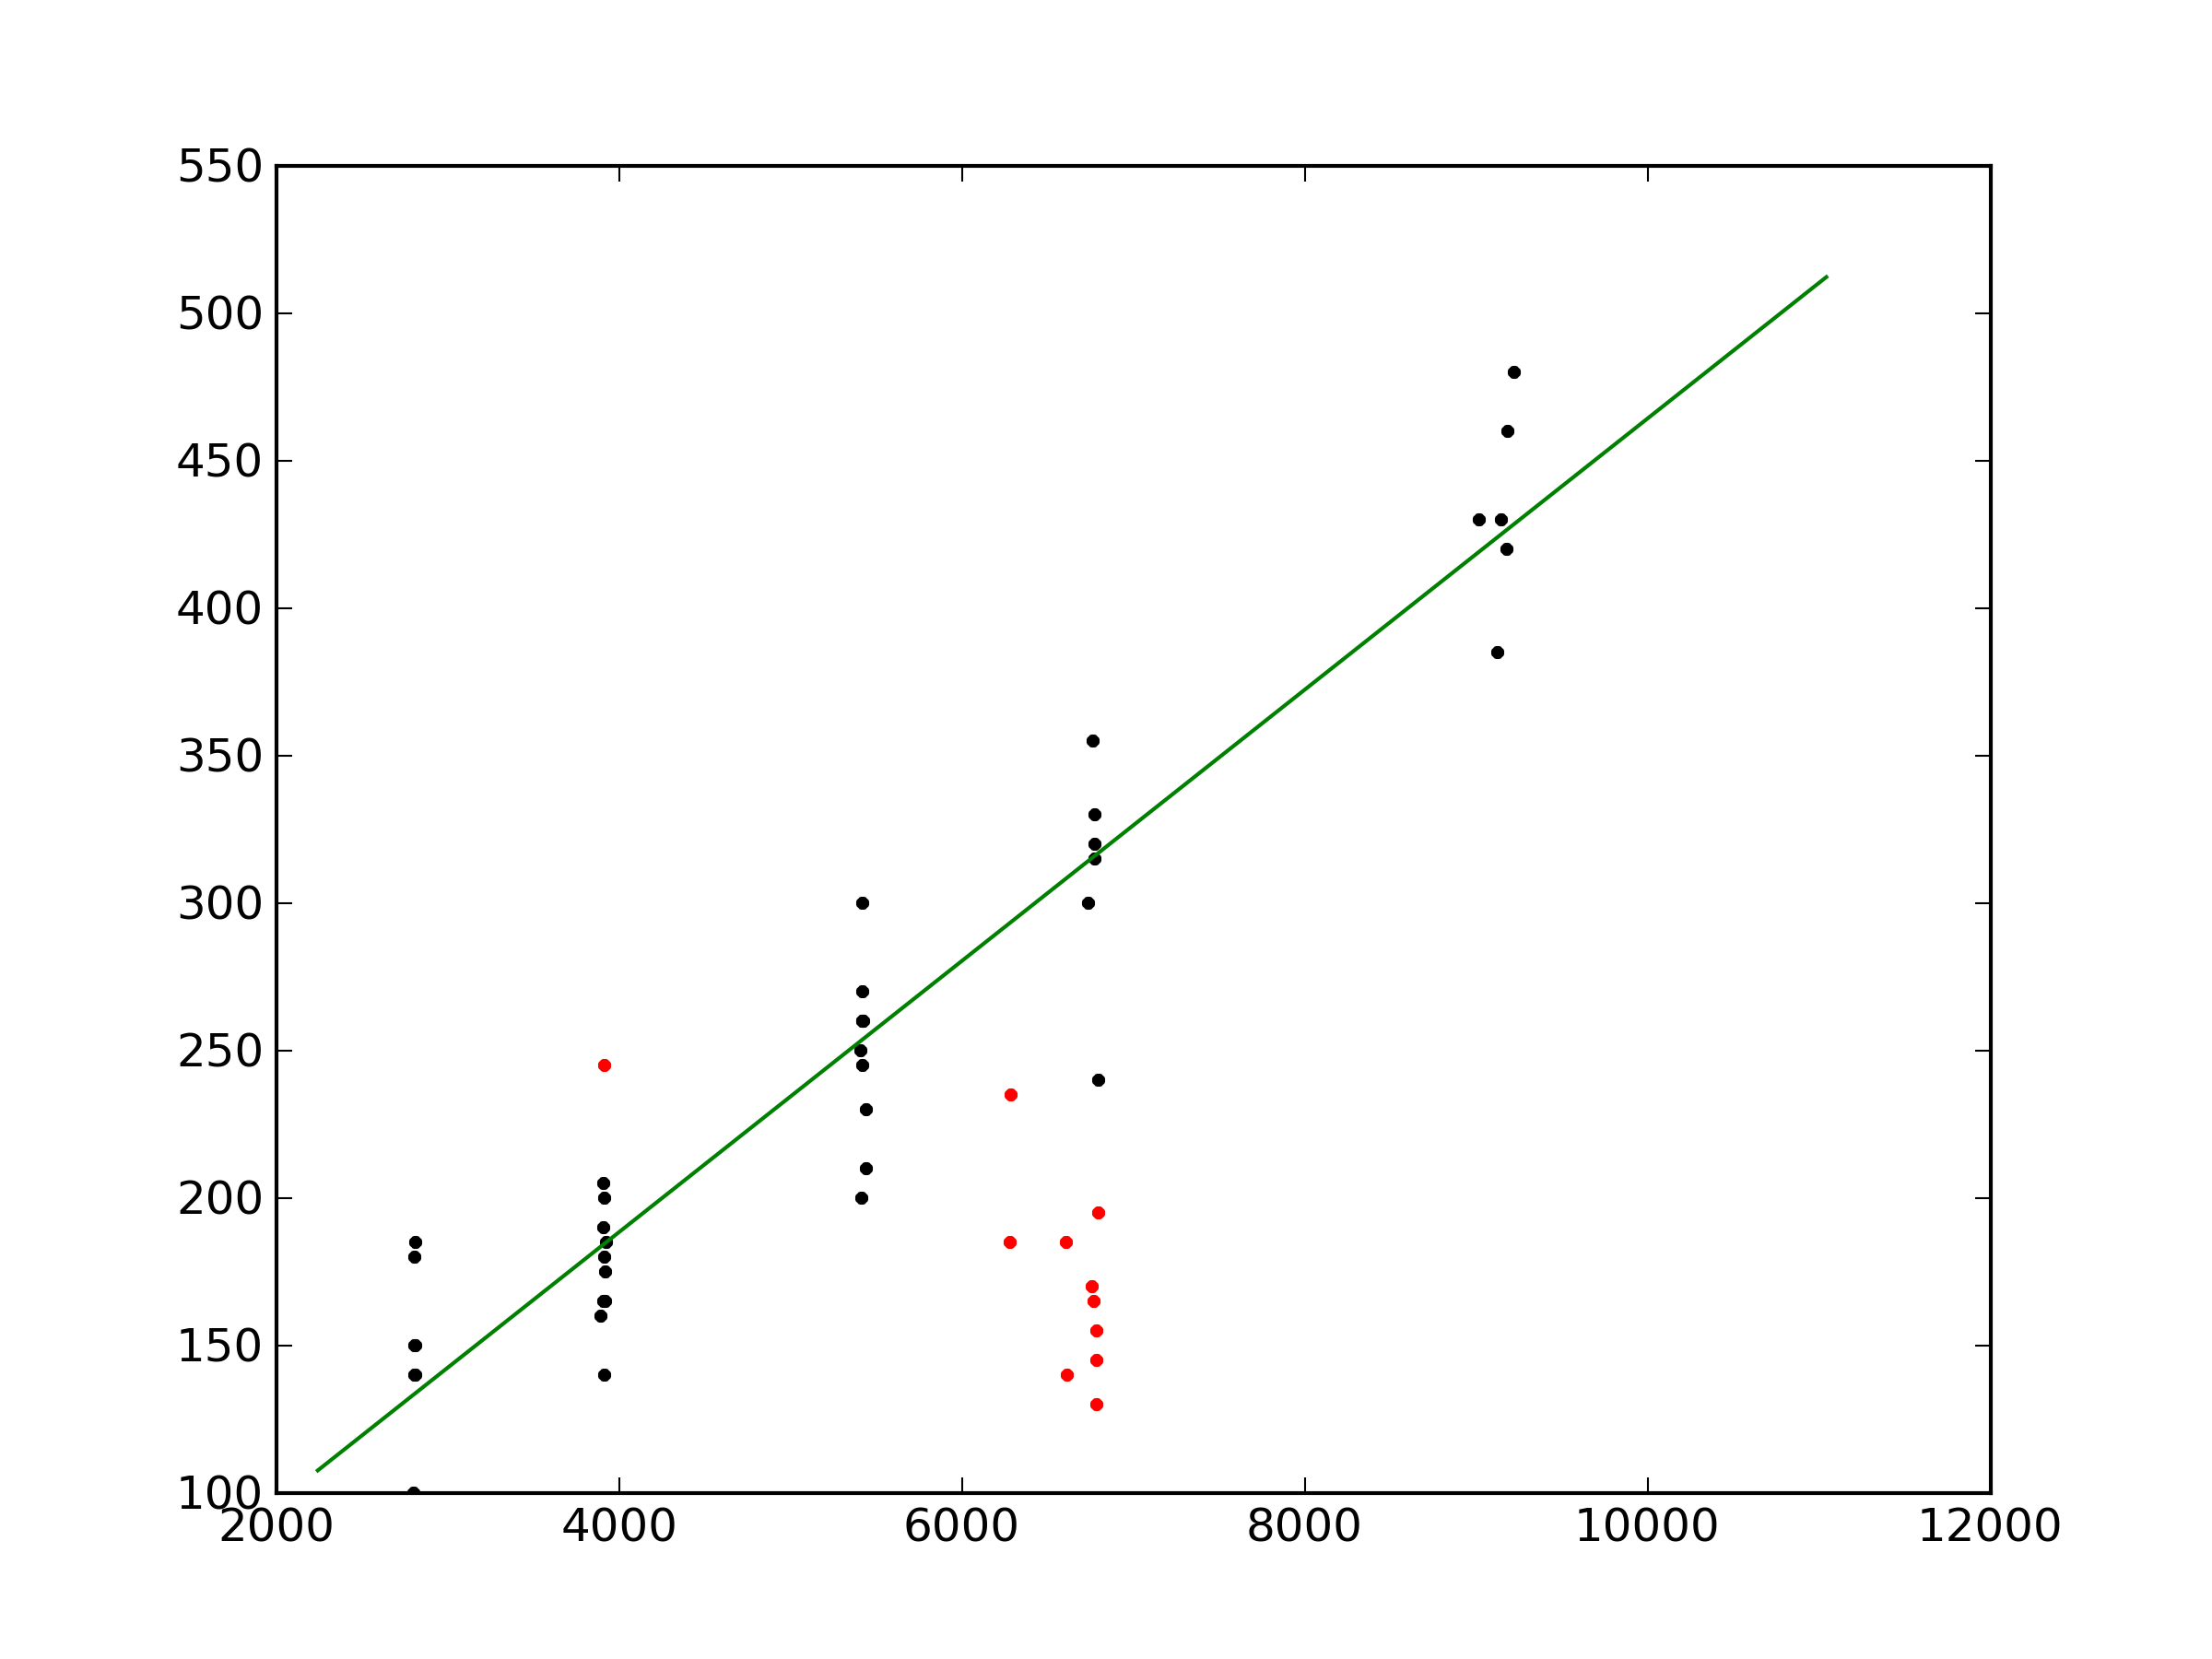
\includegraphics[scale=0.75]{grafici/C/dati.png}

\section{Analisi dati}

Chiamiamo $D = 13.480$m il cammino geometrico della luce per tornare allo specchio rotante, ovvero il doppio della distanza specchio rotante/specchio fisso; $A$ la distanza del punto di convergenza del fascio laser dalla lente $l_2$ e $B$ la distanza tra $l_2$ e lo specchio rotante. 

Per calcolare con precisione $A$, conoscendo la distanza focale di $l_2$, la ricaviamo dalla formula dei punti coniugati:
$$A=\frac{(B+D)f}{B+D-f} = 256\text{mm}$$


Per calcolare $c$, dobbiamo interpolare i dati presi nel modo seguente:
$$\Delta s = \frac{\tilde{A}}{c}\omega$$
ove
$$\tilde{A} = \frac{4*A*D^2}{2}$$

$\sage{2*e^2}$

La funzione che ci permetterà di calcolare $c$ è la seguente:

$$c = \frac{\tilde{A}}{m}$$
ove

Data una 
m=0.04594423946498933

Ricaviamo, tramite  il fit della funzione $V=R*I$" dove R è parametro da stimare, due resistenze ignote.


Misuro la resistenza interna del voltometro, mantenendo costante la ddp a $14.5\ V$ e variando la resistenza all'interno del circuito. 
Il voltmetro è in parallelo al circuito, perciò $R_i$:

$$R_i = \frac{RV}{RI-V} $$

dove R è la resistenza variabile, I la corrente nel circuito e $V= 14.5\ V$


La resistenza risulta $9.20 \pm 0.27 \ M \Omega$.


Misuriamo la resistenza interna dell'amperometro, che è collegato in serie al circuito. 

$$R_i = \frac{V-RI}{I}$$

In questo caso, R è fissato ($R=0.5 \Omega$) e sono V e I a variare

La resistenza interna risulta $11.42 \pm 0.45 \Omega$



Colleghiamo una piccola lampada a filamento al circuito, e verifichiamo che il suo comportamento resistivo non segue la legge di Ohm. 







\end{document} 



